\documentclass[
	12pt,
	BCOR=5mm,
	DIV=12,
	headinclude=on,
	footinclude=off,
	parskip=half,
	bibliography=totoc,
	listof=entryprefix,
	toc=listof,
	pointlessnumbers,
    plainfootsepline]{scrreprt}
    
% !TEX root =  master.tex

%		LANGUAGE SETTINGS AND FONT ENCODING 
%
\usepackage[ngerman]{babel} 	% German language
\usepackage[utf8]{inputenc}
\usepackage[german=quotes]{csquotes} 	% correct quotes using \enquote{}
\usepackage[T1]{fontenc}
\usepackage{lipsum}
\usepackage[hidelinks=true]{hyperref}
\usepackage{amssymb} % Math symbols
\usepackage[onehalfspacing]{setspace} % Zeileabstand
\usepackage{ gensymb }
\usepackage{ftnxtra}
\usepackage{rotating}
%\usepackage[english]{babel}   % For english language
%\usepackage{csquotes} 	% Richtiges Setzen der Anführungszeichen mit \enquote{}

% 		HYPERREF
%
% \usepackage[
% 	hidelinks=true % keine roten Markierungen bei Links
% ]{hyperref}


% Zwei eigene Befehle zum Setzen von Autor und Titel. Ausserdem werden die PDF-Informationen richtig gesetzt.
\newcommand{\TitelDerArbeit}[1]{\def\DerTitelDerArbeit{#1}\hypersetup{pdftitle={#1}}}
\newcommand{\AutorDerArbeit}[1]{\def\DerAutorDerArbeit{#1}\hypersetup{pdfauthor={#1}}}
\newcommand{\Firma}[1]{\def\DerNameDerFirma{#1}}
\newcommand{\Kurs}[1]{\def\DieKursbezeichnung{#1}}


% Correct superscripts 
\usepackage{fnpct}




%		CALCULATIONS
%
\usepackage{calc} % Used for extra space below footsepline



%		BIBLIOGRAPHY SETTINGS
%

% Uncomment the next three lines for author-year-style with footnotes (Chicago)
\usepackage[backend=biber, autocite=footnote, style=authoryear, dashed=false]{biblatex} 	%Use Author-Year-Cites with footnotes
\AdaptNoteOpt\footcite\multfootcite   %will add  separators if footcite is called multiple consecutive times 
\AdaptNoteOpt\autocite\multautocite % will add  separators if autocite is called multiple consecutive times

% Uncomment the next line for IEEE-style 
% \usepackage[backend=biber, autocite=inline, style=ieee]{biblatex} 	% Use IEEE-Style (e.g. [1])

% Uncomment the next line for alphabetic style 
% \usepackage[backend=biber, autocite=inline, style=alphabetic]{biblatex} 	% Use alphabetic style (e.g. [TGK12])

% Uncomment the next two lines vor Harvard-Style 
%\usepackage[backend=biber, style=apa]{biblatex} 	
%\DeclareLanguageMapping{german}{german-apa}


\DefineBibliographyStrings{ngerman}{  %Change u.a. to et al. (german only!)
	andothers = {{et\,al\adddot}},
}

%%% Uncomment the following lines to support hard URL breaks in bibliography 
%\apptocmd{\UrlBreaks}{\do\f\do\m}{}{}
%\setcounter{biburllcpenalty}{9000}% Kleinbuchstaben
%\setcounter{biburlucpenalty}{9000}% Großbuchstaben


\setlength{\bibparsep}{\parskip}		%add some space between biblatex entries in the bibliography
\addbibresource{bibliography.bib}	%Add file bibliography.bib as biblatex resource


%		FOOTNOTES 
%
% Count footnotes over chapters
\usepackage{chngcntr}
\counterwithout{footnote}{chapter}


%	ACRONYMS
%%%
%%% WICHTIG: Installieren Sie das neueste Acronyms-Paket!!!
%%%
\makeatletter
\usepackage[printonlyused]{acronym}
\@ifpackagelater{acronym}{2015/03/20}
  {%
    \renewcommand*{\aclabelfont}[1]{\textbf{\textsf{\acsfont{#1}}}}
  }%
  {%
  }%
\makeatother

%		LISTINGS
\usepackage{color}
\usepackage{listings}	%Format Listings properly
% Color
\definecolor{Gray}{RGB}{119, 162, 247}
\definecolor{Blue}{RGB}{209, 227, 255}
\definecolor{DarkBlue}{RGB}{38, 58, 209}
\definecolor{Green}{RGB}{184, 255, 222}
\definecolor{Red}{RGB}{255, 206, 184} 
\definecolor{DarkPurple}{rgb}{0.4,0.2,0.6}
\definecolor{GreenCom}{rgb}{0.3,0.5,0.3} 
\definecolor{OrangeString}{RGB}{212, 158, 21}
 
% \makeatletter
% \providecommand\phantomcaption{\caption@refstepcounter\@captype}
% \makeatother

\renewcommand{\lstlistingname}{Quelltext} 
\renewcommand{\lstlistlistingname}{Quelltextverzeichnis}
\lstset{numbers=left,
  numberstyle=\tiny,
  language=Java,
  frame=single,
    captionpos=b,
  basicstyle=\ttfamily\small,
  keywordstyle=\bfseries\color{DarkBlue},
  commentstyle=\itshape\color{GreenCom},
  stringstyle=\color{OrangeString},
  aboveskip=30pt,
  belowskip=30pt,
  breaklines=true
}

%		EXTRA PACKAGES
\usepackage{scrextend}
\usepackage{subfig}
\usepackage{graphicx} % use various graphics formats
\usepackage[german]{varioref} 	% nicer references \vref
\usepackage[font=onehalfspacing]{caption}	%better Captions
\usepackage{booktabs} %nicer Tabs
\usepackage{array}
%\usepackage[T1]{fontenc}
%\usepackage{amssymb}
\usepackage{algcompatible}
\usepackage{mwe}    % loads »blindtext« and »graphicx«
\usepackage{amsmath}
\usepackage{multirow}
% \usepackage{subfig}
% \usepackage{unicode-math}
% \usepackage{algorithmicx}
% \usepackage{algpseudocode}

%\newcolumntype{P}[1]{>{\raggedright\arraybackslash}p{#1}}


		% ALGORITHMS
\usepackage{algorithm}
\usepackage{algpseudocode}
% \usepackage{algorithm,algpseudocode}
\renewcommand{\listalgorithmname}{Algorithmenverzeichnis }
\floatname{algorithm}{Algorithmus}


%		FONT SELECTION: Entweder Latin Modern oder Times / Helvetica
\usepackage{lmodern} %Latin modern font
%\usepackage{mathptmx}  %Helvetica / Times New Roman fonts (2 lines)
%\usepackage[scaled=.92]{helvet} %Helvetica / Times New Roman fonts (2 lines)

%		PAGE HEADER / FOOTER
%	    Warning: There are some redefinitions throughout the master.tex-file!  DON'T CHANGE THESE REDEFINITIONS!
\RequirePackage[automark,headsepline,footsepline]{scrlayer-scrpage}
\pagestyle{scrheadings}
\renewcommand*{\pnumfont}{\upshape\sffamily}
\renewcommand*{\headfont}{\upshape\sffamily}
\renewcommand*{\footfont}{\upshape\sffamily}
\renewcommand{\chaptermarkformat}{}
\RedeclareSectionCommand[beforeskip=0pt]{chapter}
\clearscrheadfoot

\ifoot[\rule{0pt}{\ht\strutbox+\dp\strutbox}DHBW Mannheim]{\rule{0pt}{\ht\strutbox+\dp\strutbox}DHBW Mannheim}
\ofoot[\rule{0pt}{\ht\strutbox+\dp\strutbox}\pagemark]{\rule{0pt}{\ht\strutbox+\dp\strutbox}\pagemark}

\ohead{\headmark}


\begin{document}


\TitelDerArbeit{Planung und Organisation der MOBTS 2022 an der DHBW Mannheim}
\AutorDerArbeit{Tizian Groß, Tristan Emig, Anton Ochel, Benno Grimm, Anna-Lena Richert, Marcel Mertens, Marleen Benner}
\Firma{SAP SE \& Jobrouter}
\Kurs{WWI 18 SE A}

\begin{titlepage}
    
    \begin{minipage}{\textwidth}
        \vspace{5em}
        \begin{center}
            
\includegraphics[width=0.4\textwidth]{img/logo.jpg}
        \end{center}
    \end{minipage}
    \vspace{1em}
    \sffamily

    \begin{center}
        \textsf{\large{}Duale Hochschule Baden-W\"urttemberg\\[1.5mm] Mannheim}\\[2em]
        \textsf{\textbf{\Large{}Seminararbeit}}\\[3mm]
        \textsf{\textbf{\DerTitelDerArbeit}} \\[1.5cm]
        \textsf{\textbf{\Large{}Studiengang Wirtschaftsinformatik}\\[3mm] \textsf{Studienrichtung Software Engineering}}
        
        \vspace{10em}
        %\textsf{\Large{Sperrvermerk}}
    \end{center}
     
    % \begin{center}
    %     \textbf{Tizian Groß} (tizian.gross@mail.com), \textbf{Tristan Emig} (tizian.gross@mail.com) \textbf{Anton Ochel} (tizian.gross@mail.com) \textbf{Benno Grimm} (tizian.gross@mail.com) \textbf{Anna-Lena Richert} (tizian.gross@mail.com) \textbf{Marcel Mertens} (tizian.gross@mail.com) \textbf{Marleen Benner} (tizian.gross@mail.com)
    % \end{center}
    \newpage



    \begin{center}
        \vspace{5em}
        \textbf{Autoren} \\
        \DerAutorDerArbeit
        \vspace{5em}
    \end{center}
       
    
    
        \begin{minipage}{\textwidth}
    
            \begin{tabbing}
                
                Bearbeitungszeitraum: \hspace{0.85cm}\=\kill
                Kurs: \> WWI 18 SE A \\[1.5mm]
                Semester: \> 5 - 6 \\[1.5mm]
                Modul: \> Integrationsseminar \\[1.5mm]
                Studiengangsleiter: \> Prof. Dr. Sebastian Ritterbusch  \\[1.5mm]
                Dozent/-in: \> Prof. Dr. Andrea Honal \\
                \> andrea.honal@dhbw-mannheim.de \\
                \> +49 621 4105-2163 \\[1.5mm]
                Bearbeitungszeitraum: \> 15.02.2021 -- 26.04.2021
               
            \end{tabbing}
    
    \end{minipage}
    
\end{titlepage}

\pagenumbering{roman} % Römische Seitennummerierung
\normalfont

\chapter*{Kurzfassung}
\begingroup
\begin{table}[h!]
    \setlength\tabcolsep{0pt}
    \begin{tabular}{p{3.7cm}p{11.7cm}}
        Titel: & \DerTitelDerArbeit \\
        Verfasser: & \DerAutorDerArbeit \\
        Kurs: & \DieKursbezeichnung \\
    \end{tabular}
\end{table}
\endgroup


% 	Inhaltsverzeichnis
\tableofcontents

%	Abbildungsverzeichnis
\listoffigures

%	Tabellenverzeichnis
%\listoftables
%	Listingsverzeichnis
%  \lstlistoflistings

% 	Algorithmenverzeichnis
%\listofalgorithms

\clearpage
\chapter*{Abkürzungsverzeichnis}	
\addcontentsline{toc}{chapter}{Abkürzungsverzeichnis}


\begin{acronym}[RDBMS]
	\acro{DHBW}{Duale Hochschule Baden-Württemberg}
	\acro{SR}{Spektral Residuen, aus dem Engl. Spectral Residual}
	\acro{PBM}{Punktbasierte Metriken}
	\acro{SPBM}{Segmentierte Punktebasierte Metriken}
	\acro{SM}{Saliency Map}
	\acro{GT}{Grundwahrheit, aus dem Engl. Ground Truth}
	\acro{TP}{True Positives}
	\acro{FP}{False Positives}
	\acro{TN}{True Negatives}
	\acro{FN}{False Negatives}

	\acro{RDBMS}{Relational Database Management System}
	\acro{BMBF}{Bundesministerium für Bildung und Forschung}
	\acro{TSP}{Travelling Salesman Problem}	
	\acro{LE}{Längeneinheiten}
	\acro{Alg.}{Algorithmus}
	\acro{engl.}{englisch}
	\acro{SFM}{Shop Floor Management}
	\acro{OEE}{Gesamtanlageneffektivität (engl.: Overall Equiqment Effectivness)}
	\acro{MOBTS}{Management \& Organizational Behavior Teaching Society}
\end{acronym}

\ohead{Acronyms}

\clearpage
\ihead{\chaptername~\thechapter} % Neue Header-Definition (inner header)
\ohead{\headmark} % Neue Header-Definition (outer header)
\pagenumbering{arabic}  % Arabische Seitenzahlen



% BEGIN OF ACTUAL CONTENT ------------------------
\chapter{Einleitung}
\chapter{Konferenzsysteme}
Zur Verrichtung von Onlinekonferenzen können unterschiedliche Konferenzsysteme verwendete werden.
Das folgende Kapitel gibt zuerst einen Überblick über die Grundlagen von Onlinekonferenzsystemen.
Anschließend werden die Konferenzsysteme \enquote{Zoom}, \enquote{Blackboard Collaborate} und \enquote{BigBlueButton} detailliert vorgestellt.
Neben der detaillierten Vorstellung von Zoom, Blackboard Collaborate und  BigBlueButton werden Konferenzsysteme andere Hersteller kurz vorgestellt, um einen Überblick über verfügbare Konferenzlösungen zu geben.
Die detailliert vorgestellten Onlinekonferenzlösungen werden zudem auf Basis verschiedenere Merkmale wie Kosten, Skalierbarkeit oder Leistung vergleichend gegenübergestellt.
Der Vergleich kann verwendet werden, um ein geeignetes Konferenzsystem für die gegebenen Anforderungen zu finden.

\section{Grundlagen zu Konferenzsystemen}
Konferenzsysteme lassen sich in die Kategorien \textit{Videokonferenzsysteme} und \textit{Webkonferenzsysteme} einteilen.
\autocite[Vgl.][]{M_Straub.o.J.}
Auch wenn die Begriffe synonym verwendet werden, steht bei Videokonferenzen der Austausch per Video im Vordergrund.
Bei Webkonferenzen dagegen steht das Teilen von Anwendungen und das gemeinsame Zusammenarbeiten im Vordergrund.
\autocite[Vgl.][]{M_Straub.o.J.}
\\
Um an Onlinekonferenzen teilnehmen zu können, müssen einige Grundvoraussetzungen erfüllt werden.
Als Erstes wir ein Gerät benötigt, welches die Teilnahme ermöglicht.
Das kann ein Computer oder auch ein mobiles Endgerät sein.
Wenn an der Konferenz via Video teilgenommen werden soll, wird zusätzlich eine Kamera benötigt.
Mobile Endgeräte haben diese meist direkt integriert.
Für eine Audioteilnahme werden ein Mikrofon und Lautsprecher benötigt.
Statt der einzelnen Audiokomponenten kann auch ein Headset verwendet werden.
\autocite[Vgl.][]{M_Straub.o.J.}
\\
Neben den Hardwarekomponenten wird eine Internetverbindung benötigt.
Für Videokonferenzen sollte eine Bandbreite von mindestens 200 Kbits/s für den Up- und Download zur Verfügung stehen.
Des Weiteren wird ein geeignetes Onlinekonferenzsystem benötigt.
Dazu gibt es eine große Auswahl an Onlinekonferenzwerkzeugen.
\autocite[Vgl.][]{M_Straub.o.J.}
\\
Mit Videokonferenzen kann eine effiziente Zusammenarbeit mit Personen auf der ganzen Welt erreicht werden.
Digitale Treffen bieten viele Möglichkeiten, die ein persönliches Treffen in einigen Bereichen ersetzen können.
\autocite[Vgl.][]{M_Mierke.2020}
\\
Onlinekonferenzen helfen zudem bei der Einsparung von Reisezeit sowie der Einsparung von gefahrenen oder geflogenen Kilometern.
Auch können Personen an Konferenzen teilnehmen, die gleichzeitig Kinder betreuen müssen oder denen die Einreise verwehrt worden ist.
\autocite[Vgl.][]{M_Sladek.2020}
\\
In der Wirtschaft spielen Online-Seminare und Konferenzen eine große Rolle.
Mitarbeiter und Führungskräfte können durch den Einsatz von digitalen Konferenzen und Schulungen weitergebildet werden.
Onlineschulungen helfen dabei, dass das Personal keine zusätzliche Arbeitszeit benötigt und keine Reisekosten hat, um an einer Schulung teilnehmen zu können.
\autocite[Vgl.][]{M_GrunderkucheRedaktion.2021}
\\
Im IT-Bereich nutzen Hersteller eigene Onlineschulungen oft auch dazu, um Kunden anzuwerben.
\autocite[Vgl.][]{M_GrunderkucheRedaktion.2021}
Es gibt für das Abhalten von Onlinekonferenzen verschieden Möglichkeiten:\\
Konferenzen können dabei als Videokonferenz, als Liveevent oder als vorher aufgenommene Session abgehalten werden.
Je nach gewählter Präsentationsmethode können Zuschauer unterschiedlich mit der Konferenz interagieren.
\autocite[Vgl.][]{M_Sladek.2020}
\\
Sollen Diskussionen oder Workshops durchgeführt werden, können nur Videokonferenzen abgehalten werden.
Teilnehmer sollten für eine erfolgreiche Teilnahme an Workshops eine gute Audioqualität haben.
Zudem ist es sinnvoll, dass Onlinediskussionen moderiert werden.
Für eine bessere Zuordnung der Sprecher kann es hilfreich sein, dass Teilnehmer ein Profilbild von sich bereitstellen oder per Video an der Diskussion teilnehmen.
Diese Art von Onlinekonferenzen eignet sich vor allem für geringe Teilnehmerzahlen.
\autocite[Vgl.][]{M_Sladek.2020}
\\
Eine andere Möglichkeit für Onlinekonferenzen ist das Livestreamen von Events.
Dabei wird ein Event mit einer geringen Verzögerung an eine große Anzahl an Zuschauer übertragen.
\autocite[Vgl.][]{M_Sladek.2020}
\\
Ein Nachteil von Livestreaming ist die Voraussetzung einer stabilen und schnellen Internetverbindung.
\autocite[Vgl.][]{M_Maciej.2016}
Wenn eine stabile Internetverbindung nicht gewährleistet werden kann, bietet es sich an, vorher Inhalte aufzunehmen und als Video bereitzustellen.
Zudem können Teilnehmer so selber entscheiden, zu welchem Zeitpunkt sie welche Inhalte konsumieren.
Es kann zudem dafür gesorgt werden, dass Inhalte barrierefrei bereitgestellt werden.
So können zum Beispiel vorher Untertitel erzeugt und für die Videos bereitgestellt werden.
\autocite[Vgl.][]{M_Sladek.2020}
\\
Zwischenmenschliche Kommunikation kann jedoch nicht komplett durch digitale Konferenzen ersetzt werden.
Das Kennenlernen anderer Personen und das Schließen von neuen Bekanntschaften ist im Rahmen von Onlinekonferenzen fast nicht möglich.
Es kann für einige Teilnehmer schwierig sein, andere Konferenzteilnehmer per Chat anzuschreiben und ein Gespräch aufzubauen.
\autocite[Vgl.][]{M_Sladek.2020}
\\
Anhand dieser Informationen wird deutlich, dass Onlinekonferenzen einige Vorteile bieten, aber auch Nachteile haben.
Sie eignen sich vor allem dazu, einem großen Publikum über zum Teil große Distanzen neue Inhalte zu vermitteln, dabei bleibt die zwischenmenschliche Kommunikation aber oft auf der Strecke.
Für die digitale Fernlehre bieten Onlinekonferenzen und Seminare jedoch ein großes Potential.
Entscheidend für die digitale Lehre ist der richtige Einsatz der gegebene Werkzeuge.

\section{Konferenzsysteme vorgestellt}
\label{sec:konferenzsysteme_vorgestellt}
\subsection{Zoom}
Zoom ist eine von der \textit{Zoom Video Communications Inc.} bereitgestellte Lösung für Onlinekonferenzen.
\autocite[Vgl.][]{M_Zoom.o.J.b}
In der kostenlosen Variante von Zoom können bis zu 100 Teilnehmer an einer Videokonferenz teilnehmen.
Sobald sich mehr als drei Personen in einer Sitzung befinden, wird die maximale Sitzungsdauer auf 40 Minuten begrenzt.
Um eine längere Sitzungsdauer zu ermöglichen, ist es notwendig, die kostenpflichtige Version von Zoom zu verwenden.
Damit kann die Sitzungsdauer auf bis zu 24 Stunden verlängert werden. Die Kosten dafür betragen 13,99 Euro pro Monat pro Moderator.
Ein Moderator stellt bei Zoom einen Gastgeber für eine Onlinekonferenz dar.
Um einen Schutz vor unberechtigtem Betreten von Meetings zu ermöglichen, können Zoommeeting mit einem Passwortschutz versehene werden.
So können nur Teilnehmer mit dem entsprechenden Passwort an einer Onlinekonferenz teilnehmen.
\autocite[Vgl.][]{M_Mierke.2020}
\\
Neben den genannten Funktionen können Teilnehmer von Zoommeetings bis zu 49 Videos pro Bildschirm sehen.
Das Teilnehmerlimit für eine Sitzung liegt bei 1000 Teilnehmern.
Um Inhalte wie Präsentationen zu teilen, bietet Zoom Teilnehmern die Möglichkeit, ihren Bildschirm freizugeben.
Die Funktion kann dabei von mehreren Teilnehmern gleichzeitig genutzt werden, sodass in einem Meeting mehrerer Bildschirme zur selben Zeit geteilt werden können.
Um ein Meeting auch für Teilnehmer bereitzustellen, die Internetprobleme haben oder die verhindert sind, können Meetings aufgezeichnet werden.
\autocite[Vgl.][]{M_Zoom.o.J.b}
\\
Teilnehmer können mit verschiedenen Endgeräten an Zoommeetings teilnehmen.
Dazu kann eine entsprechende Anwendung auf einem Computer oder mobilen Endgerät installiert werden.
Zoom bietet Desktop-Clients für die Betriebssyteme Windows, MacOS und Linux an.
Für mobile Endgeräte wie Tablets oder Smartphones bietet Zoom Applikationen für die Betriebssysteme Android und iOS an.
Neben der Nutzung des Zoom-Clients auf einem Endgerät können Teilnehmer auch über ihren Webbrowser an Meetings teilnehmen.
\autocite[Vgl.][]{M_Zoom.o.J.}

\subsection{Blackboard Collaborate}
Blackboard Collaborate ist eine von \textit{Blackboard Inc.} bereitgestellte Onlinekonferenzlösung, die vor allem auf die Onlinelehre abzielt.
\autocite[Vgl.][]{M_Blackboard.o.J.}
Blackboard Collaborate gibt an, besonders für die Bildung gemacht zu sein und auf die Bedürfnisse von Lehrenden und Lernenden angepasst zu sein.
Dazu bietet Blackboard Collaborate die Möglichkeit, direkt aus dem Webbrowser heraus nutzbar zu sein.
Der Download eines besonderen Clients wird dabei nicht benötigt.
Wie bei Zoom gibt es auch bei Blackboard Collaborate verschiedene Lizenzen, die mehr oder weniger Funktionen zur Verfügung stellen.
Es wird zwischen der Enterprise und der Departmentlizenz unterschieden.
Die Departmentlizenz bietet die Möglichkeit, dass bis zu 500 Teilnehmer an einer Konferenz teilnehmen können.
Zusätzlich können bis zu 500GB an Dateien gespeichert werden. Die Sitzungszeit ist auf 1000000 Minuten begrenzt.
Die Enterpriselizenz bietet wie die Departmentlizenz maximal 500 Teilnehmern die Möglichkeit, an einer Onlinesitzung teilzunehmen.
Die Speicher- und Sitzungszeitbegrenzungen sind jedoch Variable.
Die Kosten für die Departmentlizenz betragen 9000 Dollar pro Jahr, für die Enterpriselizenz wird ein individueller Preis gezahlt, der von den gewünschten Funktionen abhängt.
\autocite[Vgl.][]{M_Blackboard.o.J.}
\\
Das Blackboard Collaborate kann auf verschiedene Weisen genutzt werden.
Es gibt die Möglichkeit, wie in einem Klassenraum den Teilnehmern eine Anwendung zu teilen und Dinge zu präsentieren.
Zudem können Teilnehmer in kleineren Gruppen zusammenarbeiten.
\autocite[Vgl.][]{M_Blackboard.o.J.}
\\
Auch besteht die Möglichkeit, Umfragen zu erstellen oder virtuell die Hand zu heben.
Auf diese Weise können Lehrende mit den Lernenden interagieren und Feedback erhalten.
Neben der Möglichkeit einer Sitzung mit einer Internetverbindung beizutreten, bietet Blackboard Collaborate die Möglichkeit, per Telefon an einer Sitzung teilzunehmen.
Dabei kann jedoch nur die Audiofunktion genutzt werden.
Falls die eigene Audioeingabe nicht funktionieren sollte, kann der integrierte Chat zur Kommunikation zwischen den Teilnehmern einer Sitzung genutzt werden.
Die Nutzung des digitalen Whiteboards kann Lehrenden dabei helfen, Dinge wie an einer Tafel zu visualisieren.
\autocite[Vgl.][]{M_NorthernIllinoisUniversity.o.J.}

\subsection{BigBlueButton}
BigBlueButton ist wie Blackboard Collaborate ein Onlinekonferenzwerkzeug mit dem Fokus auf digitalem Lernen.
Genau wie Blackboard Collaborate ist BigBluebutton vor allem ein Webkonferenzsystem, welches in einem Webbrowser verwendet werden kann.
BigBlueButton ist zudem ein Open Source Projekt.
\autocite[Vgl.][]{M_BigBlueButton.o.J.b}
\\
Bei Open Source Projekten ist der Programmcode für alle Menschen einsehbar.
Das bietet den Vorteil, dass Menschen aus der ganzen Welt an dem Projekt mitentwickeln können.
Durch Open Source können Fehler schneller entdeckt und behoben werden.
Zudem können Programme an individuelle Bedürfnisse angepasst werden.
\autocite[Vgl.][]{M_RedHat.o.J.}
\\
BigBlueButton bietet wie Blackboard Collaborate verschiedene Nutzungsmöglichkeiten.
Lehrende können beispielsweise ein digitales Whiteboard nutzen, um Dinge zu visualisieren.
Die Zeichnungen können von den Sitzungsteilnehmern in Echtzeit verfolgt werden.
Um zwischenmenschliche Kommunikation zu ermöglichen, können alle Teilnehmer per Videofeed an der Sitzung teilnehmen.
Es gibt dabei kein Limit, wie viele Teilnehmer ihre Kamera nutzen können.
Das einzige Limit ist die Internetbandbreite der Teilnehmer.
\autocite[Vgl.][]{M_BigBlueButton.o.J.}
\\
BigBlueButton bietet neben dem Teilen von Inhalten und halten von Videokonferenzen die Möglichkeit zu chatten, Emojis zu verwenden, Umfragen zu starten sowie zusammen an Whiteboards zu arbeiten.
Zudem können sogenannte \enquote{Breakout Rooms} erstellt werden, um so in kleineren Gruppen zusammenarbeiten zu können.
\autocite[Vgl.][]{M_BigBlueButton.o.J.}
\\
Im Gegensatz zu Zoom ist BigBlueButton kein direkt nutzbarere Service.
Um BigBlueButton nutzen zu können, muss ein eigener Server verwendet werden, auf dem die Software installiert wird.
Auch ist es notwendig, die gewünschten Einstellungen selbst vorzunehmen, sodass auch hier Zeit und personelle Ressourcen benötigt werden.
Der Vorteil an einer selbst gehosteten Lösung ist jedoch die Kontrolle über die anfallenden Daten.
Zudem kann der Serverstandort selbst bestimmt werden.
So kann die Verarbeitung von personenbezogenen Daten in Deutschland oder der Europäischen Union gewährleistet werden.
\autocite[Vgl.][]{M_Klicksafe.o.J.}

\subsection{Weitere Onlinekonferenzsysteme}
Neben den vorgestellten Lösungen für Onlinekonferenzen existiert eine Vielzahl weiterer Anwendungen.
Diese Werkzeuge sind dabei auf die unterschiedlichen Anwendungsfälle und Bedürfnisse der Benutzer angepasst.
Im Folgenden wird eine kleine Übersicht über weitere Onlinekonferenzsysteme und ihre Einsatzmöglichkeit gegeben.
Die Werkzeuge werden dabei nicht so detailliert behandelt wie die in \autoref{sec:konferenzsysteme_vorgestellt} vorgestellten Lösungen.
\\
Einige Hersteller der im Folgenden genannten Werkzeuge bieten aufgrund von Corona eigentlich kostenpflichtige Funktionen zur kostenlosen Nutzung an.
\autocite[Vgl.][]{M_Straub.o.J.}

\subsubsection{Skype}
Um Skype nutzen zu können, wird ein Skype-Account benötigt.
Es können kostenlos Anrufe mit bis zu 50 Teilnehmern durchgeführt werden.
Ein Nachteil von Skype sind häufige Störungen in der Übertragung.
\autocite[Vgl.][]{M_Straub.o.J.}
\\
Neben einer privaten Lizenz könne Firmen \textit{Skype for Business} verwenden.
\autocite[Vgl.][]{M_Microsoft.o.J.}

\subsubsection{Google Meet}
\textit{Meet} ist eine von Google zur Verfügung gestellte Videokonferenzlösung.
Sie funktioniert über den Webbrowser und ist kostenpflichtig.
Dazu kann eine Unternehmenslizenz erworben werden.
Nur Teilnehmer mit einer Lizenz können Meetings organisieren, die Teilnahme an organisierten Meetings kann jedoch auch ohne eine eigene Lizenz erfolgen.
Meet ist in Googles \textit{G Suite} integriert, daher lassen sich Termine und Kontakte einfach importieren
\autocite[Vgl.][]{M_Straub.o.J.}

\subsubsection{Microsoft Teams}
Microsoft Teams beinhaltet neben der Videokonferenzfunktion einen Chat sowie die Möglichkeit, Dateien auszutauschen.
Zudem lassen sich Microsoft-Anwendungen wie \textit{Excel}, \textit{Word} und \textit{Power Point} direkt in Teams nutzen.
Dateien werden über \textit{Microsoft Sharepoint} allen Teilnehmern einer Gruppe bereitgestellt.
Die Planung von Meetings kann mit \textit{Outlook} und dem Werkzeug \enquote{Planner} erfolgen.
Teams ist für bis zu 300 Teilnehmer kostenlos, es können jedoch auch kostenpflichtige Unternehmenslizenzen erworben werden.
\autocite[Vgl.][]{M_Straub.o.J.}

\subsubsection{Bitrix 24}
Bitrix 24 eignet sich vor allem für kleine Firmen und bietet umfassende Möglichkeiten zur Projekt- und Aufgabenplanung.
Es gibt sechs unterschiedliche Lizenzen, von denen eine kostenlos ist.
In der kostenlosen Version können bis zu zwölf Teilnehmer an einem Meeting teilnehmen.
\autocite[Vgl.][]{M_Straub.o.J.}

\subsubsection{Mikogo}
Mikogo ist hauptsächlich für das Teilen von Bildschirmen geeignet.
Es bietet sowohl eine kostenlose als auch eine kostenpflichtige Version an.
Die kostenlose Version ermöglicht es mit bis zu 25 Teilnehmern zu kommunizieren.
Mikogo ermöglicht es zudem Dokumente zu teilen, Sitzungen aufzuzeichnen und ein virtuelles Whiteboard zur Verfügung zu stellen.
Es ist vollständig webbasiert, was den Download zusätzlicher Software überflüssig macht.
\autocite[Vgl.][]{M_Straub.o.J.}

\section{Vergleich der Konferenzsysteme}
Die folgende Tabelle stellt den Vergleich der Konferenzsysteme \textit{Zoom}, \textit{Blackboard Collaborate} und \textit{BigBlueButton} zusaamenfassend dar:
\begin{table}[H]
    \centering
    \resizebox{0.97\textwidth}{!}{%
    \begin{tabular}{l|lll}
        & \textbf{Zoom}                                                                                                                                                                        & \textbf{\begin{tabular}[c]{@{}l@{}}Blackboard\\ Collaborate\end{tabular}}                                                                                                                                                                                                             & \textbf{BigBlueButton}                                                                                                                                                                                                     \\ \hline
        Anbieter                                                                                 & \begin{tabular}[c]{@{}l@{}}Zoom Video \\ Communications Inc.\end{tabular}                                                                                                            & Blackboard Inc.                                                                                                                                                                                                                                                                       & BigBlueButton                                                                                                                                                                                                              \\ \hline
        Abgestimmt auf                                                                           & \begin{tabular}[c]{@{}l@{}}Digitale\\ Zusammenarbeit\end{tabular}                                                                                                                    & Onlinelehre                                                                                                                                                                                                                                                                           & Onlinelehre                                                                                                                                                                                                                \\ \hline
        Direkt betriebsbereit?                                                                   & Ja                                                                                                                                                                                   & Ja                                                                                                                                                                                                                                                                                    & Muss selbst gehostet werden                                                                                                                                                                                                \\ \hline
        \begin{tabular}[c]{@{}l@{}}Datenschutz-\\ konform?\end{tabular}                          & n. a.                                                                                                                                                                                & n. a.                                                                                                                                                                                                                                                                                 & \begin{tabular}[c]{@{}l@{}}Kann DSGVO-\\ konform verwendet\\ werden\end{tabular}                                                                                                                                           \\ \hline
        Funktionen                                                                               & \begin{tabular}[c]{@{}l@{}}- Audio \& Video Funktionen\\ - Bildschirm- \& Anwendungs-\\ freigabe für Teilnehmer\\ - Aufzeichnen von Sitzungen\\ - Chat\\ - Gruppenräume\end{tabular} & \begin{tabular}[c]{@{}l@{}}- Audio \& Video Funktionen\\ - Bildschirm- \& Anwendungs-\\ freigabe für Teilnehmer\\ - Aufzeichnen von Sitzungen\\ - Digitales Whiteboard\\ - Gruppenräume\\ - Teilnahme via\\ Telefonverbindung\\ - Umfragen\\ - Digitales melden\\ - Chat\end{tabular} & \begin{tabular}[c]{@{}l@{}}- Audio \& Video Funktionen\\ - Bildschirm- \& Anwendungs-\\ freigabe für Teilnehmer\\ - Aufzeichnen von Sitzungen\\ - Digitales Whiteboard\\ - Gruppenräume\\ - Umfragen\\ - Chat\end{tabular} \\ \hline
        \begin{tabular}[c]{@{}l@{}}Maximale Teilnehmer-\\ anzahl pro Sitzung\end{tabular}        & \begin{tabular}[c]{@{}l@{}}- In der kostenlosen\\ Version: 100\\ - Mit kostenpflichtiger\\ Lizenz: 1000\end{tabular}                                                                 & \begin{tabular}[c]{@{}l@{}}- Mit Departmentlizenz: 500\\ - Mit Enterpriselizenz: 500\end{tabular}                                                                                                                                                                                     & Kein Teilnehmerlimit                                                                                                                                                                                                       \\ \hline
        \begin{tabular}[c]{@{}l@{}}Maximale\\ Sitzungsdauer\end{tabular}                         & \begin{tabular}[c]{@{}l@{}}- In der kostenlosen\\ Version: 40 Minuten\\ - Mit kostenpflichtiger\\ Lizenz: 24 Stunden\end{tabular}                                                    & \begin{tabular}[c]{@{}l@{}}- Bei Departentlizenz:\\ 1000000 Minuten\\ - Bei Enterpriselizenz:\\ variabel\end{tabular}                                                                                                                                                                 & n. a.                                                                                                                                                                                                                         \\ \hline
        Software-Lizenz                                                                          & Closed Source                                                                                                                                                                        & Closed Source                                                                                                                                                                                                                                                                         & Open Source                                                                                                                                                                                                                \\ \hline
        \begin{tabular}[c]{@{}l@{}}Unterstützte\\ Betriebssysteme \& \\ Plattformen\end{tabular} & \begin{tabular}[c]{@{}l@{}}- MacOS\\ - Windows\\ - Linux\\ - iOS\\ - Android\\ - Webbrowser\end{tabular}                                                                             & Webbrowser                                                                                                                                                                                                                                                                            & Webbrowser                                                                                                                                                                                                                 \\ \hline
        Kosten                                                                                   & \begin{tabular}[c]{@{}l@{}}13,99 Euro pro\\ Moderator pro Monat\end{tabular}                                                                                                         & \begin{tabular}[c]{@{}l@{}}- Departmentlizenz:\\ 9000 Dollar pro Jahr\\ - Enterpriselizenz:\\ Preis auf Anfrage\end{tabular}                                                                                                                                                          & \begin{tabular}[c]{@{}l@{}}Software selbst ist\\ kostenlos, es fallen\\ jedoch Kosten für\\ Server an.\end{tabular}
    \end{tabular}%
    }
    \caption[Vergleich Onlinekonferenzsysteme]{Vergleich von Zoom, Blackboard Collaborate und BigBlueButton.}
    \label{tab:vergleich_online_konferenzsysteme}
\end{table}

Wie \autoref{tab:vergleich_online_konferenzsysteme} zeigt, unterscheiden sich die unterschiedlichen Konferenzsysteme in ihrem Funktionsumfang meist nur geringfügig.
Alle drei vorgestellten Systeme können zum digitalen Zusammenarbeiten mit Audio und Videofunktionen verwendet werden.
Blackboard Collaborate und BigBlueButton besitzen einige Funktionen, die besonders auf die Onlinelehre angepasst sind.
Die Kosten der Systeme unterscheiden sich im Gegensatz zu den Funktionen stark.
Auch gibt es Unterschiede in Bezug auf die direkte Nutzbarkeit der Systeme.
Zoom und Blackboard Collaborate bieten die Möglichkeit, direkt nutzbar zu sein.
BigBlueButton muss dagegen selbst installiert werden.
Der Vorteil daran ist jedoch, dass der Speicherort der Daten besser kontrolliert werden kann als bei direkt nutzbaren Systemen, die von den Anbietern bereitgestellt werden.
\chapter{Eventmanagement}
\section{Einführung}
Events beziehungsweise Veranstaltungen sind in den letzten Jahren zu einem der bedeutendsten Marketinginstrumenten sowohl für Unternehmen, Organisationen als auch Privatpersonen aufgestiegen. Sie ermöglichen und fördern den Aufbau einer starken, persönlichen und emotionalen Beziehung zwischen den Veranstaltern und der dazugehörigen Kundenzielgruppe, was insgesamt zu einer besseren und dauerhafteren Kundenbindung führt. Ebenso bilden diese real Events einen kreativen Gegenpol zur voranschreitenden Digitalisierung, was durch die vermehrten virtuellen Konversationen und Begegnungen mit anderen Mitmenschen, Arbeitskollegen oder Stakeholdern von jedem einzelnen wahrgenommen werden kann.\autocite[Vgl.][]{Eventmanagementstudieren.de.o.J.}

Mit der globalen Ausbreitung des Covid-19 Virus mussten allerdings die meisten, wenn nicht sogar alle Events abgesagt oder auf unbestimmte Zeit verschoben werden, wie beispielsweise die Fußball Europameisterschaft 2020 oder auch die weltweit wichtigste sicherheitspolitische Konferenz, welche jährlich Anfang des Jahres in München stattfindet. 
Nur die allerwenigsten Veranstaltungen sind durch ein virtuell stattfindendes Event ersetzt worden, was auf die Notwendigkeit dieser einzelnen Veranstaltungen zurückzuführen ist, wie unteranderem der G7-Gipfel.\autocites[Vgl.][]{Tagesschau.o.J.}[Vgl.][]{Nahar.o.J.}

Das Eventmanagement beinhaltet alle notwendigen Aktivitäten für die erfolgreiche Durchführung eines Events. Es übernimmt also die Aufgaben der Zielsetzung, operativen Planung und Durchführung in einem vorgegebenen Rahmen. Im Eventmanagement steht stets der Kunde im Mittelpunkt, weshalb das Eventmanagement stark von subjektiven sowie psychologischen Aspekten geprägt ist.\autocite[Vgl.][]{ZeitOnline.o.J.}

\section{Begriff: Event}
Der Begriff \enquote{Event} hat seinen Ursprung im englischen Sprachraum und wird mit \enquote{Ereignis} oder auch \enquote{Veranstaltung} übersetzt. Aufgrund der stark subjektiven Wahrnehmung von Events gibt es in der Theorie und Praxis keine einheitliche und genaue Definition. Dennoch kann ein Event durch folgende zentrale Charakteristiken beschrieben werden: 

\begin{itemize}
    \item Erinnerungswert
    \item Einzigartig- und Einmaligkeit
    \item Aktivierung der Besucher, Positivität
    \item Planung, Organisation und Inszenierung
    \item erlebnisorientierten Ereignis
\end{itemize}

Mit diesem allgemeinen Verständnis von Events beziehungsweise Veranstaltungen soll nun die mögliche Kategorisierung von Events dargelegt werden. 

\begin{table}[!h]
    \centering
    \begin{tabular}{l|l}
        \textbf{Event-Cluster}      & \textbf{Beispiel} \\ \hline
        Kultur-Event                & Open-Air-Konzert, Festival, königliche Hochzeit        \\ \hline
        Sport-Event                 & Super-Bowl, Fußball-WM, Olympia   \\ \hline
        ökonomisches Event          & Apple Keynote, Hauptversammlung   \\ \hline
        politisches Event           & G7-, G20-Gipfel, Münchner Sicherheitskonferenz                   \\ \hline
        natürliches Event           & Sonnenfinsternis, Sternschnuppen        
    \end{tabular}%
    \caption{}
    \label{tab:event-cluster}
\end{table}

Eine dieser Systematisierungen besteht in der Unterteilung von Veranstaltungen basierend auf ihrer Größe. So klassifiziert der Autor Walter Freyer Events in Mega-, Medium- und Mikro-Events. Neben dieser einfachen Art der Systematisierung können Veranstaltungen aufgrund ihres Anlasses geclustert werden, wie in \autoref{tab:event-cluster} verdeutlicht. Eine Einheitliche Kategorisierung von Events gibt es aufgrund des subjektiven Aspekts erneut nicht. Deshalb wäre ebenso die Kategorisierung in Kommerzielle und Nicht-Kommerzielle Events eine korrekte Unterteilung von Events.\autocite[Vgl.][S. 23 ff.]{Eisermann.2014}

Ein Event wird aus einem bestimmten Grund geplant und durchgeführt. Deshalb sollte zu Beginn das Ziel bzw. der Zweck des Events festgehalten werden und während des gesamten Eventmanagementprozesses im Kopf behalten werden. Das jeweilige Ziel eines Events kann sehr unterschiedlich ausfallen und kann unter anderem sein:

\begin{itemize}
    \item Finanzieller Effekt
    \item Einfluss auf Personen
    \item Steigerung der Bekanntheit
    \item Akquirierung von Sponsoren und Teilnehmern
\end{itemize}

Von diesen primären Zielen eines Events lassen sich die sekundären Ziele ableiten. Mögliche sekundären Ziele sind eine hohe Besucherzahl oder auch eine starke Medienpräsenz. Insgesamt ist jedes Event am Ziel und folglich am Kunden / Besucher orientiert. Zum Erreichen dieses Ziels wird bei einem Event mit der Emotionalen Ebene gearbeitet, um die Teilnehmer zu erreichen. Deshalb ist ein Event stark subjektiv.\autocite[Vgl.][S. 6 ff.]{Holzbaur.2002}

\section{Aufgaben des Eventmanagement}
Das Eventmanagement umfasst alle Aufgaben der Planung, Organisation, Überwachung und Steuerung, die bei der Ausführung eines Events notwendig sind. Grundsätzlich wird ein Event wie ein Projekt geplant und durchgeführt, weshalb wesentliche Prinzipien des Projektmanagements ebenso im Eventmanagement beachtet werden müssen. Aus diesem Grund soll an dieser Stelle das magische Dreieck des Projektmanagements vorgestellt werden.\autocite[Vgl.][S. 22]{Holzbaur.2002}

Das magische Dreieck, dargestellt in \autoref{fig:EM_magisches_Dreieck}, besteht aus drei Ecken, die die drei Hauptmerkmale des Projekts repräsentieren:

\begin{figure}[H]
    \centering
    \setlength{\fboxsep}{10pt}
    \setlength{\fboxrule}{0.5pt}
    \fbox{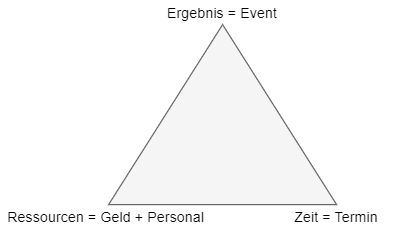
\includegraphics[width=0.65\textwidth]{img/EM_MagischesDreieck.png}}
    \caption[Eventmanagement: magisches Dreieck]{Darstellung des magischen Dreiecks aus dem Projektmanagements. (Quelle: In Anlehnung \autocite[]{Holzbaur.2002})} \label{fig:EM_magisches_Dreieck}
\end{figure}

\textbf{Ergebnis:} 
\\
Das Hauptmerkmal Ergebnis ist im Eventmanagement das Event selbst und stellt das oberste Ziel des Projektes dar. Wie bereits im oberen Abschnitt beschrieben lassen sich über das Event Sekundärziele ableiten. Beispielsweise ist das Primärziel die Veranstaltung eines Freundschaftsspiels zwischen einem großen und kleinen Fußballclub. Neben dem Sportereignis an sich, kann die Vorstellung eines Königstransfers oder das Aufbessern der Vereinskasse die Sekundärziele sein.

\textbf{Ressourcen:}
\\
Das Hauptmerkmal Ressourcen beinhaltet die monetären Mittel, die Infrastruktur wie Räumlichkeiten und Parkplätze sowie das Personal und Arbeitszeit. Die Ressourcen stellen also alle notwenigen Aufwendung während des gesamten Projekts dar.

\textbf{Zeit:}
\\
Das Hauptmerkmal Zeit oder im Eventmanagement Termin ist primär der Zeitpunkt der Ausführung des Events. Darüber hinaus zählt zu diesem Hauptmerkmal selbstverständlich auch das Einhalten von davor geplanten Terminen, wie unteranderem das rechtzeitige Plakatieren, versenden der Einladungen oder Verkauf von Event-Tickets.

Auch im Eventmanagement weisen die drei Hauptmerkmale Wechselwirkungen auf. So muss beispielsweise beim Ausfall von Personal während der Planung und Organisation des Events, das Hauptmerkmal der Zeit oder des Ergebnisses diese Veränderung im Hauptmerkmal der Ressourcen kompensieren. 

Aufgrund des Projektcharakters kann  ein Event in Meilensteine und Projektphasen unterteilt werden, wie in \autoref{fig:EM_PH_MS} veranschaulicht:

\begin{figure}[H]
    \centering
    \setlength{\fboxsep}{10pt}
    \setlength{\fboxrule}{0.5pt}
    \fbox{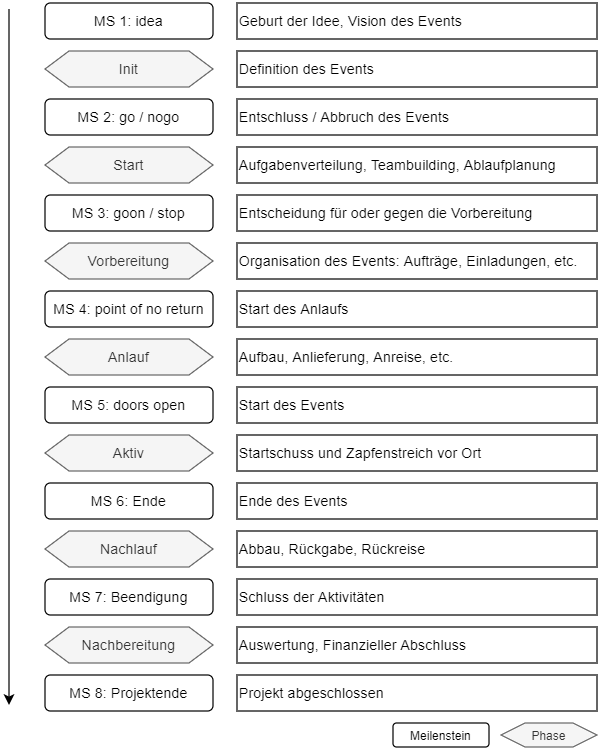
\includegraphics[width=0.7\textwidth]{img/EM_PH_MS.png}}
    \caption[Eventmanagement: Meilensteine und Phase eines Events]{Darstellung der acht Meilensteine und sieben Phasen bei der Veranstaltung eines Events. (Quelle: In Anlehnung \autocite[Vgl.][S. 23]{Holzbaur.2002})} \label{fig:EM_PH_MS}
\end{figure}

Die hier aufgezeigten Meilensteine und Phasen stehen in einer engen Beziehung zu einander und können gemeinsam als Grundlage eines Terminplans dienen. Die Termine und Dauer der jeweiligen Meilensteine und Phasen kann von Event zu Event stark variieren. Beispielsweise ist die Phase Aktiv eines Open-Air-Konzerts nur einige Stunden lang, wohingegen bei einem Musik-Festival diese Phase mehrere Tage dauert. Grundsätzlich leiten sich die Termine der Meilensteine von der Dauer den jeweiligen Phasen ab. Der Terminplan kann in einer einfachen Tabelle, Gantt-Diagramm oder ähnlichen Formen abgebildet werden.\autocite[Vgl.][S. 24 ff.]{Holzbaur.2002}

Neben der Gliederung eines Events in Meilensteinen und Phasen empfiehlt es sich zudem innerhalb des Projektes (Events) eine organisatorische sowie inhaltliche Struktur aufzubauen.

Die organisatorische Projektstruktur ist meist eine hierarchische Aufteilung in Aufgabenbereiche bzw. Teilprojekte. Mit dieser Aufteilung werden für verschiedene Bereiche Verantwortliche und Ansprechpartner sichergestellt. Eine grobe Projektorganisation innerhalb eines Events kann in \autoref{fig:EM_Aufbauorganisation} betrachtet werden. 

\begin{figure}[H]
    \centering
    \setlength{\fboxsep}{10pt}
    \setlength{\fboxrule}{0.5pt}
    \fbox{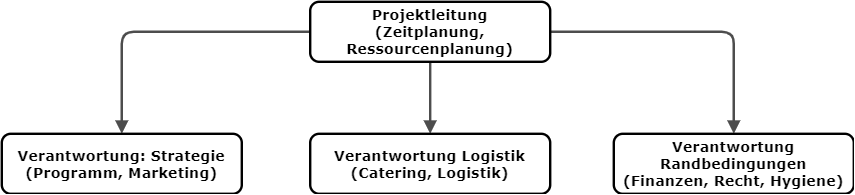
\includegraphics[width=0.8\textwidth]{img/EM_ORG.png}}
    \caption[Eventmanagement: Aufbauorganisation]{Darstellung einer High-Level Aufbauorganisation (Quelle: Eigene Darstellung} \label{fig:EM_Aufbauorganisation}
\end{figure}

Die inhaltliche Projektorganisation im Eventmanagement kann über den Projektstrukturplan PSP\autocite[]{projektmanagementdefinitionen.de.o.J.} erreicht werden. In diesem werden sämtliche Tätigkeiten eines Events aufgenommen. Tätigkeiten stellen dabei die kleinste Arbeitseinheit dar. Mehrere Tätigkeiten können wiederum zu einem Arbeitspaket zusammengefasst werden und Arbeitspakete können letztlich zu Teilprojekte zusammengefasst werden.\autocite[Vgl.][S. 144 f.]{Holzbaur.2002}

Mit Hilfe des Strukturplans erhalten die Verantwortlichen eine bessere Übersicht über die einzelnen Aufgaben und Arbeitspakete. Zudem unterstützt der Strukturplan den Projektleiter bei Controlling spezifischen Aufgaben.

Nachdem ein grober Überblick über die Projektstruktur sowie Meilensteine und Eventphasen gegeben worden ist soll nun die verschiedenen Aufgabenbereiche innerhalb eines Events genauer betrachtet werden. Wie bereits in Abbildung dargelegt können drei Hauptaufgabenbereiche ausgemacht werden: Strategie, Logistik und Randbedingungen. 

\textbf{Strategie:}

Der Aufgabenbereich der Strategie befasst sich mit den Themen Marketing und Programm. Die Kernaufgabe besteht in der Zieldefinition des Events. Nachdem dieses Ziel festgelegte wurde muss anschließend ein passendes Eventprogramm entwickelt werden. Hierfür muss eine Zielgruppe definiert werden und eine sorgfältige Analyse des Markts durchgeführt werden, um ein erfolgreiches Programm zu entwerfen. Ein mögliches Eventprogramm wird in einem folge Kapitel vorgestellt. Neben der Erstellung des Eventprogramms ist eine weitere wesentliche Aufgabe die Ausarbeitung einer passenden Marketingkampagne. Beispiele solcher Marketingmaßnahmen sind Werbevideos oder auch Broschüren. Allerdings müssen je nach Event und Zielgruppe entsprechende Kommunikationswege ausgewählt werden. Die letzte wesentliche Aufgabe dieses Bereichs besteht in der Suche nach einem möglichen Sponsoring. Diese Aufgabe kann allerdings je nach Event entfallen.

\textbf{Logistik:}

Der Aufgabenbereich der Logistik beinhaltet alle Tätigkeiten, die einen reibungslosen Ablauf eines Events sicherstellt. Die erste und wichtigste Aufgabe besteht in der Festlegung der Eventlocation. Diese muss selbstverständlich abhängig des Eventziels und Eventgröße ausgewählt werden. Des Weiteren organisiert der Aufgabenbereich der Logistik das Catering, die Aufteilung der Räumlichkeiten und für eine eventuelle Bereitstellung von Transportmöglichkeiten wie beispielsweise vom Flughafen zur Eventlocation. Auch die Müllentsorgung ist Teilaufgabe dieses Aufgabenbereichs und sollte bei der Planung eines Events nicht unberücksichtigt bleiben.

\textbf{Randbedingungen:}

Der Aufgabenberiech der Randbedingungen hat drei Hauptaufgaben. Die erste dieser besteht in der rechtlichen Absicherung. Beispielsweise können Genehmigung der Stadt notwendig sein, um ein Event an einem Sonntag ausführen zu dürfen. Die zweite Aufgabe besteht in der Ausarbeitung eines Sicherheits- sowie Gesundheitskonzepts. Sowohl die Sicherheit als auch Gesundheit muss während eines Events sichergestellt werden. Durch die Entwicklungen in den letzten Jahren durch verschiedene Attentate aber auch durch Corona-Pandemie steigt die Wichtigkeit dieser beiden Aspekte. Durch die Ausarbeitung solcher Konzepte kann in Notsituationen auf diese zurückgegriffen werden und möglicherweise schlimmeres verhindern. Die dritte Hauptaufgabe besteht in der Überwachung der Finanzen und Wirtschaftlichkeit des Events, wie beispielsweise die Buchführung.

Neben diesen drei Aufgabenbereichen kann auch das Projektmanagement als solches gewertet werden. Allerdings würde eine ausführliche Erläuterung der Aufgaben des Projektmanagements den Rahmen dieser Arbeit sprengen, weshalb auf eine genauere Ausarbeitung verzichtet wird und auf die zahlreiche Literatur, die dieses Thema behandelt, hingewiesen.

\chapter{Imagefilm}
\section{Film, eine Einleitung}
\begin{quote}
    Ein Bild sagt mehr als tausend Worte
\end{quote}
\begin{flushright}
    Fred R. Barnard
\end{flushright}
Mit diesem Zitat lässt sich die Wichtigkeit des Films als kommunikationsmittel sehr gut beschreiben. So liefert ein Film nicht nur eine große Menge an Informationen durch Darstellung eines Bildes, sondern kann ein Film auch zeitliche Abläufe vermitteln. Oft haben Filme auch noch das weitere Medium des Tons, welches in sich nochmals mehr Informationen trägt. Ein Film kann deswegen als ein sehr \enquote{dichtes} Informationsträger angesehen werden, da in kurzer Zeit sehr viele Informationen gleichzeitig, teils durch verschiedene Kanäle wie Bild und Ton, übertragen werden. So ergibt auch der Einsatz dieses Mediums für die \ac{MOBTS} Konferenz in Mannheim Sinn.\\

Im Folgendem wird deshalb kurz die Geschichte des Films erläutert, um die Vorteile und die interessante Herkunft dieses Mediums darzustellen. Anschließend wird auf verschiedene Techniken des Filmens eingegangen, welche die Grundlagen der Filmproduktion darstellen. Danach wird auf die Umsetzung des Werbefilms für die \ac{MOBTS} Konferenz eingegangen, welcher anschließend bewertet wird. Zuletzt wird noch in einem Fazit ein kurzer Ausblick gegeben.
\section{Geschichte des Films}
Der Mensch suchte schon seit Ewigkeiten danach, seine Erfahrungen und Erlebnisse visuell darzustellen. So finden sich schon in den frühesten Zivilisationen verschiedenste Darstellungen der Umwelt. Noch bevor der Mensch Schrift erfand malte er auf Höhlenwände Bilder. Mit dem technischen Fortschritt entwickelte sich auch die Darstellungsformen, sodass Bilder auf Leinwände gemalt wurden, bis schließlich die Fotografie erfunden wurde. Bei der Fotografie wird ein lichtempfindlicher Film durch eine Linse mit Licht bestrahlt, was ein Abbild der Umwelt darstellt.\\
Um das Bild bewegt erscheinen zu lassen, erzeugt ein Film eine Illusion, indem mehrere aufeinanderfolgende Bilder schnell hintereinander dargestellt werden. Dies erscheint dann aber einer Bildrate von 24 Bildern pro Sekunde dem menschlichen Auge als flüssige Bewegung.\autocite{Schmidt.2013}\\
Auf der Suche nach dem allerersten \enquote{Film} gibt es drei wesentliche Kandidaten.\autocite{HeadsUp.} Der chronologisch erste Film wurde 1878 erstellt.\autocite{Muybridge.1878} Das Ziel dieses Films war es, herauszufinden, ob ein Pferd im Gallopp jemals mit allen vier Hufen gleichzeitig den Boden verlässt. Dafür Fotografierte Edward Muybridge ein Pferd in Palo Alto, Kalifornien im Lauf mehrfach mit verschiedenen Kameras, die entlang der Strecke aufgestellt waren. Diese verschiedenen Fotos wurden dann im Nachhinein schnell hintereinander gezeigt, um zu entdecken, dass ein Pferd mit allen vier Hufen gleichzeitig vom Boden abhebt. Hier war es jedoch nicht die Absicht von Muybridge, ein Bewegtbild zu erzeugen, weshalb dies oft nicht als erster Film angesehen wird.\\
Oft wird der Film Roundhay Garden Scene als der erste Film betitelt.\autocite{LePrince.1888} Der von Louis Amie Augustin Le Prince erstellte Film von 1888 geht zwar lediglich zwei Sekunden, stellt jedoch schon eine zusammenhängende Handlung dar und gilt deswegen als Film.\\
Etwas länger dagegen ist der Film \enquote{Arrival of a Train at A la Ciotat}, im original \enquote{L'Arrivée d'un Train A la Ciotat}, welcher 1895 von den Gebrüdern Lumiere erstellt wurde.\autocite{Lumiere.1895} Dieser 50-sekündige Film zeigt einen einfahrenden Zug, eine bekannte Alltagsszene. Zu diesem Film gibt es die unbestätigte Geschichte, welche besagt, dass die Zuschauer dieses Films von der Illusion in einem solchen Sinne getäuscht wurden, sodass sich Panik breit machte und einige Zuschauer aus Angst aus dem Theater flohen. Auch wenn diese Geschichte vielleicht nicht wahr ist, zeigt sie die Überzeugungskraft des Mediums und die Emotionen, die durch visuelle Einflüsse ausgelöst werden können.\\
Dieses Ziel blieb ein wichtiges Ziel in der Filmkunst und Regisseure versuchen bis heute, wirksam Emotionen in Zuschauern auszulösen.\\
So gab es einige wichtige Regisseure, welche die Filmindustrie zu dem machten, was sie heute ist.
\section{Techniken des Filmens}
\subsection{Framing}
\subsection{Goldener Schnitt}
\subsection{Skript und Storyboard}
\subsection{Schnitte und Übergänge}
\subsection{Voiceover}
\section{Imagefilm zur MOBTS}
\subsection{Ziel des Films}
\subsection{Skript des Films}
\subsection{Storyboard des Films}
\subsection{Durchführung und Produktion}
\section{Bewertung und Reflektion}
\section{Fazit und Ausblick}
\chapter{Konferenzplanung}
\section{Einführung}
Die MOBTS-Konferenz 2022 wird an der DHBW in Mannheim stattfinden \autocite[Vgl.][]{MOBTS.04.03.2021}. Das folgende Konzept richtet sich an die Verantwortlichen der DHBW, die sich um die Umsetzung der Konferenz kümmern. Mithilfe des Konzepts soll die erfolgreiche Vorbereitung und Ausführung der Konferenz an der DHBW Mannheim unterstützt sowie wichtige Informationen für die Teilnehmer zusammengetragen werden. Durch die MOBTS-Konferenz sollen den Teilnehmern wichtige Vorträge und Informationen bezüglich des Themas \enquote{Digital Learning} näher gebracht werden. Das Thema ist vor allem in der heutigen digitalen Zeit ein sehr wichtiges Gebiet. Die Zielgruppen des Events sind Personen, die im Lehrbereich tätig sind, Studenten und Schüler, die vom digitalen Lernen betroffen sind oder auch Personen, die sich allgemein für das Thema interessieren. Auch das Thema \enquote{Remote Working} kann verknüpft werden, weswegen auch Führungskräfte zu der Zielgruppe zählen.
 
Im Folgenden werden die Rahmenbedingungen der Konferenz definiert. Diese findet von Donnerstag, den 23. Juni bis Sonntag, den 26. Juni statt, wobei am ersten und letzten Tag keine Vorträge, Workshops und Debatten geplant sind. Wie bereits erwähnt fokussiert sich die Konferenz auf das Thema \enquote{Digital learning}. Hierzu werden sich im Rahmen der Konzeptplanung mögliche Unterthemen und Sprecher überlegt, die an der Konferenz Vorträge halten könnten. Die Konferenz soll in den Räumen der D- und E-Gebäude der DHBW stattfinden. Es werden ungefähr 150 Teilnehmer erwartet, plus circa 20 Tagesgäste, die mit Essen und Trinken versorgt werden sollen. Die Kosten sollen sich allerdings im Rahmen halten, damit die Ticketkosten nicht 200 EUR pro Person übersteigen. Außerdem wird eine Online-Teilnahme angeboten, für die die Ticketkosten natürlich geringer werden. Hier werden weitere 100 Teilnehmer erwartet, wodurch mit einer Gesamtteilnahme von ungefähr 250 Personen gerechnet wird. Da die Konferenz-Teilnehmer aus aller Welt kommen, werden alle Dokumente, die die Teilnehmer über die Konferenz informieren sowie wichtige Hinweise liefern auf Englisch erstellt. Zu diesen Dokumenten gehört unter anderem ein FAQ, mit dem Fragen beantwortet werden, die bei den Teilnehmern aufkommen könnten, ein Anfahrtsplan zur DHBW vom Frankfurter und Stuttgarter Flughafen und welche Zusatzevents es in Mannheim und Heidelberg neben der Konferenz gibt. Außerdem wird ein Flyer mit den wichtigsten Informationen sowie eine Umfrage erstellt, die die Teilnehmer nach der Konferenz beantworten sollen. Da im Moment noch nicht abzusehen ist, wie die Corona-Lage im Konferenz-Jahr 2022 aussehen wird, ist es außerdem wichtig, ein Hygienekonzept für die Konferenz zu erstellen, damit die Veranstaltung regelkonform ablaufen kann.

\section{Themen und Sprecher}
Wie bereits erwähnt liegt der Fokus der Konferenz auf dem Thema \enquote{Digital Learning}. Im Anhang \vref{app:konferenzthemen} ist eine vollständige Liste möglicher Unterthemen zu finden, über die auf der Konferenz ein Vortrag gehalten werden könnte. Zu den Themenvorschlägen gehören unter anderem \enquote{Gamification}, \enquote{Digital Schools} und \enquote{Digital Learning @ DHBW}.

Des Weiteren wurden verschiedene Sprecher recherchiert, die möglicherweise einen Vortrag zum Thema \enquote{Digital Learning} halten könnten. Dazu gehört unter anderem der Chief Learning Officer der SAP, Max Wessel, sowie Jill Grinager vom Hasso-Plattner-Institut. Eine vollständige Liste der möglichen Sprecher kann in Tabelle\vref{tab:speaker} gefunden werden. Des Weiteren sollen noch Speaker gesucht werden, die einen Online-Vortrag halten und während der Konferenz nicht an der DHBW Vorort sind. 

\begin{table}[]
	\centering
	\resizebox{\textwidth}{!}{%
		\begin{tabular}{|l|l|l|}
			\hline
			\textbf{Name}          & \textbf{Unternehmen/Institution} & \textbf{Kontakt}              \\ \hline
			Max Wessel             & SAP                              & max.wessel@sap.com            \\ \hline
			Prof. Dr. Nagler       & DHBW                             & georg.nagler@dhbw-mannheim.de \\ \hline
			Jill Grinager          & HPI                              & jill.grinager@hpi.de          \\ \hline
			Johanna Schulz         & HPI                              & johanna.schulz@hpi.de         \\ \hline
			Maren Metz             & HFH                              & maren.metz@hamburger-fh.de    \\ \hline
			Dr. Michael Wache      &                                  & michael-wache.de              \\ \hline
			Prof. Dr. Andrea Honal & DHBW                             & andrea.honal@dhbw-mannheim.de \\ \hline
			Doro Moritz            & GEW                              & doro.moritz@gew-bw.de         \\ \hline
			Maire Landsberg        & BVMW                             & marie.landsberg@bvmw.de       \\ \hline
		\end{tabular}%
	}
	\caption{Vorgeschlagene Speaker für die MOBTS-Konferenz}
	\label{tab:speaker}
\end{table}

\section{Ablauf der Konferenz}
Der komplette Ablauf der Konferenz kann in Tabelle \vref{tab:konferenzablauf} angeschaut werden. 

\begin{table}[h]
	\centering
		\begin{tabular}{|l|l|l|}
			\hline
			\textbf{Datum}              & \textbf{Zeit} & \textbf{Event}                                                                                        \\ \hline
			23.06.2022                  & 16:30 - 20:30 & \begin{tabular}[c]{@{}l@{}}Begrüßung und Kennenlernen, \\ anschließend gemeinsames Essen\end{tabular} \\ \hline
			\multirow{7}{*}{24.06.2022} & 7:30          & Registration am Helpdesk                                                                              \\ \cline{2-3} 
			& 7:30 - 8:30   & Kaffee, Snacks to go                                                                                  \\ \cline{2-3} 
			& 8:30 - 9:30   & Eröffnungsrede                                                                                        \\ \cline{2-3} 
			& 9:45 - 13:00  & Sessions, workshops etc.                                                                              \\ \cline{2-3} 
			& 13:00 - 13:45 & Mittagspause                                                                                          \\ \cline{2-3} 
			& 13:45 - 17:15 & Sessions, workshops etc.                                                                              \\ \cline{2-3} 
			& 18:00         & Stadtführung                                                                                          \\ \hline
			\multirow{6}{*}{25.06.2022} & 8:00 - 8:30   & Kaffee, Snacks to go                                                                                      \\ \cline{2-3} 
			 & 8:30 - 9:00   & Eröffnungsrede                                                                                        \\ \cline{2-3} 
			& 9:00 - 13:00  & Sessions, workshops etc.                                                                              \\ \cline{2-3} 
			& 13:00 - 13:45 & Mittagspause                                                                                          \\ \cline{2-3} 
			& 13:45 - 16:00 & Sessions, workshops etc.                                                                              \\ \cline{2-3} 
			& 16:15 - 17:15 & Abschluss                                                                                             \\ \cline{2-3} 
			& 17:45         & Gemeinsames Essen                                                                                     \\ \hline
		\end{tabular}%
	\caption{Ablauf der Konferenz}
	\label{tab:konferenzablauf}
\end{table}
Die Teilnehmer kommen voraussichtlich am Donnerstag, den 23. Juni in Mannheim an. In der DHBW ist in dem Raum neben dem AudiMax dann bereits ein Tisch aufgebaut, bei dem sich die Teilnehmer registrieren können und eine Willkommens-Tüte mit verschiedenen Goodies und ihr Namensschild abholen können. Um 16:30 Uhr kann sich am Wasserturm oder an einer anderen Location zu einer kleinen Begrüßung und einem vorzeitigen Kennenlernen getroffen werden, wobei die Teilnahme hierfür selbstverständlich freiwillig ist. Hier sollte jedoch ein Ort gewählt werden bei dem genug Platz für alle Teilnehmer wäre.

Freitags haben ab 7:30 Uhr die Teilnehmer, die sich donnerstags noch nicht registriert hatten, noch einmal die Möglichkeiten dies nachzuholen. Gleichzeitig gibt es Kaffee und ein paar Snacks, bei denen die Teilnehmer noch einmal die Möglichkeit haben sich zu unterhalten oder zu frühstücken, bevor dann von 8:30 Uhr – 9:30 Uhr die Eröffnung der Konferenz folgt. Diese übernimmt Prof. Dr. Nagler im Raum Audi Max, da hier 200 Plätze zur Verfügung stehen und somit alle Teilnehmer einen Platz finden. Daraufhin folgt eine 15 Minuten Pause, bevor es dann mit den Vorträgen, Workshops und Debatten weitergeht. Diese dauern jeweils ungefähr eineinhalb Stunden. Mittags, von 12 Uhr bis 13 Uhr ist eine Mittagspause eingeplant. Hierfür werden im Raum über dem Audi Max verschiedene Finger Foods aufgebaut. Nach der Pause finden bis 17 Uhr weitere Sessions statt. Eine genauere Planung der verschiedenen Sessions ist hierbei erst möglich, wenn die Anzahl der Sprecher sowie die verschiedenen Themen feststehen. Erst dann ist ebenso eine endgültige Raumeinteilung möglich. In \autoref{tab:sessionablauf}
ist allerdings dargestellt, wie ein möglicher Ablauf der Konferenz mit den Unterthemen, die sich im Rahmen des Konzeptes überlegt wurden, aussehen kann. Für abends (von 18 Uhr – 20:30 Uhr) ist ein freiwilliges Event für die Teilnehmer geplant. Dies könnte zum Beispiel eine Stadtführung sein, damit die Teilnehmer auch Mannheim kennen lernen können.
 
Samstags startet der Konferenz-Tag ab 8:30 Uhr. Hier folgt bis 9 Uhr eine kleine Begrüßung zum zweiten Tag und anschließend starten wieder die verschiedenen Sessions mit den Workshops, Präsentationen und Debatten mit Unterbrechungen von jeweils 15 Minuten Pausen. 

Um einen Teil der Konferenz online ablaufen zu lassen, müssen in jedem Raum Kameras aufgestellt werden, die den Vortrag über eine Videokonferenz-Plattform wie zum Beispiel Zoom übertragen. Hier macht es Sinn, jemanden bei einem Laptop zu platzieren, der den Vortrag online verfolgt und die Fragen der digitalen Teilnehmer an den Vortragenden weiterleiten kann.
 
Falls es zur Zeit der Konferenz immer noch Corona-Einschränkungen gibt, macht es möglicherweise Sinn, die verschiedenen Sessions so zu planen, dass die 15 Minuten Pausen zwischen den verschiedenen Sessions nicht auf den selben Zeitpunkt fallen, um die Begegnungen geringer zu halten. Dadurch entsteht allerdings der Nachteil, dass eine Session erst endet, wenn eine andere bereits begonnen hat, wodurch die Teilnehmer in ihrer Wahl nicht mehr so flexibel sind.

\begin{table}[]
	\centering
		\begin{tabular}{|l|*{3}{>{\centering\arraybackslash}p{6cm}|}}
			\hline
			\textbf{Zeit} & \textbf{Raum A}                                    & \textbf{Raum B}                                                                                                   \\ \hline
			9:45          & \multirow{5}{*}{Digital Schools}                   & \multirow{5}{*}{Remote working}                                                                                   \\ \cline{1-1}
			10:00         &                                                    &                                                                                                                   \\ \cline{1-1}
			10:15         &                                                    &                                                                                                                   \\ \cline{1-1}
			10:30         &                                                    &                                                                                                                   \\ \cline{1-1}
			10:45         &                                                    &                                                                                                                   \\ \hline
			11:00         & Kaffeepause                                        & Kaffeepause                                                                                                       \\ \hline
			11:15         & \multirow{4}{*}{Digital Learning @ DHBW}           & \multirow{4}{*}{Duale Ausbildung International}                                                                   \\ \cline{1-1}
			11:30         &                                                    &                                                                                                                   \\ \cline{1-1}
			11:45         &                                                    &                                                                                                                   \\ \cline{1-1}
			12:00         &                                                    &                                                                                                                   \\ \hline
			12:15         & \multicolumn{2}{c|}{\multirow{3}{*}{Mittagspause}}                                                                                                                     \\ \cline{1-1}
			12:30         & \multicolumn{2}{c|}{}                                                                                                                                                  \\ \cline{1-1}
			12:45         & \multicolumn{2}{c|}{}                                                                                                                                                  \\ \hline
			13:00         & \multirow{4}{*}{Gamification}                      & \multirow{4}{*}{Motivation im digitalen Zeitalter}                                                                \\ \cline{1-1}
			13:15         &                                                    &                                                                                                                   \\ \cline{1-1}
			13:30         &                                                    &                                                                                                                   \\ \cline{1-1}
			13:45         &                                                    &                                                                                                                   \\ \hline
			14:00         & Kaffeepause                                        & Kaffeepause                                                                                                       \\ \hline
			14:15         & \multirow{5}{*}{\begin{tabular}[c]{@{}c@{}}Moocs / Online Corporate \\ Learning\end{tabular}} & \multirow{5}{*}{\begin{tabular}[c]{@{}c@{}}Social / Personal Development im \\ Online Zeitalter\end{tabular}}     \\ \cline{1-1}
			14:30         &                                                    &                                                                                                                   \\ \cline{1-1}
			14:45         &                                                    &                                                                                                                   \\ \cline{1-1}
			15:00         &                                                    &                                                                                                                   \\ \cline{1-1}
			15:15         &                                                    &                                                                                                                   \\ \hline
			15:30         & Kaffeepause                                        & Kaffeepause                                                                                                       \\ \hline
			15:45         & \multirow{6}{*}{Pädagogik für Dozenten}            & \multirow{6}{*}{\begin{tabular}[c]{@{}c@{}}Digitalisierung in der Hochschule \\ in Bezug auf Corona\end{tabular}} \\ \cline{1-1}
			16:00         &                                                    &                                                                                                                   \\ \cline{1-1}
			16:15         &                                                    &                                                                                                                   \\ \cline{1-1}
			16:30         &                                                    &                                                                                                                   \\ \cline{1-1}
			16:45         &                                                    &                                                                                                                   \\ \cline{1-1}
			17:00         &                                                    &                                                                                                                   \\ \hline
		\end{tabular}%
	\caption{Ein beispielhafter Ablauf eines Konferenztages.}
	\label{tab:sessionablauf}
\end{table}

\section{Hygienekonzept}
Da die Corona-Lage im Jahre 2022 noch nicht vorher gesagt werden kann ist es wichtig, das Hygienekonzept immer an die aktuellen Vorgaben anzupassen. Dabei sollte darauf geachtet werden wie viele Personen an der Konferenz teilnehmen dürfen, um eventuell auf eine mehrheitlich digitale Konferenz umzusteigen. Des Weiteren sollten die allgemeinen Regeln eingehalten werden. So sollten die Besucher einen Mund-Nasen-Schutz tragen, wenn diese nicht an ihrem Platz sitzen oder gerade am Essen oder Trinken sind. Die Stühle in den Konferenzsälen sollten mit einem Abstand von mindestens 1,5 Meter Abstand zueinander aufgestellt werden. In Räumen, in denen es feste Sitze gibt, wie im Audi Max, sollten die Plätze die nicht belegt werden dürfen abgesperrt werden, um einen ausreichenden Abstand zu gewährleisten. Während den 15 Minuten Pausen zwischen zwei Sessions sollte der Raum durchgelüftet und gereinigt werden. Außerdem macht es Sinn, bei einer Ansammlung von einer großen Anzahl von Person auf einem engen Raum auch während der Session Fenster aufzumachen, falls es die Wetterlage erlaubt. Des Weiteren sollten ausreichend Desinfektionsmittelspender aufgestellt werden, damit die Teilnehmer sich die Hände desinfizieren können. Ebenso sollte ein separater Aus- und Eingang zu den Konferenzgebäuden zur Verfügung gestellt werden. So kann der eigentliche Eingang in Gebäude D weiterhin als Eingang verwendet werden, während die Tür beim Audi Max als Ausgang fungieren kann. Daher sollten auch verschiedene Schilder erstellt werden, die auf den Eingang und Ausgang hinweisen. Ebenfalls sollte es Schilder geben, die auf die verschiedenen Hygieneregeln hinweisen, wie die Mundschutzpflicht, die Husten- und Niesetikette, den ausreichenden Abstand, dass Händeschütteln vermieden und sich regelmäßig die Hände desinfiziert werden sollte. Eine weitere Vorsichtsmaßnahme ist es, ein Einbahnstraßensystem zu definieren und die Wege so abzukleben, damit die Teilnehmer den benötigten Abstand einhalten können. Auch sollten so viel Aktivitäten wie möglich draußen geplant werden, weswegen es Sinn macht, dass die Teilnehmer in den 15 Minuten Pausen möglicherweise nach draußen vor das Gebäude gehen, da hier auch mehr Platz zur Verfügung steht. 

\section{Catering}
Für die Verpflegung der Teilnehmer über die zwei Konferenz-Tage soll ein Catering bereitgestellt werden. Dieses soll im Raum über dem Audi Max aufgebaut werden, wodurch es nah an den Session-Räumen und somit leicht und schnell zu erreichen ist. Für das Catering wurde ein Angebot von Peters Party Service eingeholt (siehe Anhang \vref{app:angebot}). In dem Angebot bietet dieser Mittagessen von 11:30 - 14 Uhr an. Geschirr, Besteck sowie Servietten werden hierbei von ihm bereitgestellt. An Tag eins hätte dieser als warme Option eine Kartoffelsuppe mit Gemüsestreifen und als kalte Optionen verschiedenes Fingerfood. Darunter Mini-Bifteki, Mini-Frikadellen, Falaffelbällchen und Käse-Obstspieße. Falls gewünscht würde er außerdem um 14:30 Uhr ein Blechkuchen-Mix anbieten, was in die 15-Minuten Pausen nachmittags gelegt werden könnte. Am zweiten Tag wird als warme Speise eine ungarische Gulaschsuppe angeboten sowie als kalte Option belegte Partyrötchen, Mini-Frühlingsrollen, Blätterteighappen, Capresespieße, Frischkäse-Pasteten sowie gegrilltes, eingelegtes Gemüse. Als Dessert kann außerdem Panna Cotta oder Mousse au chocolat bestellt werden. Zusätzlich kann dieser verschiedene Getränke bereitstellen. Eine Frühstücksoption, wie zum Beispiel verschiedenes Laugengebäck, wird von seinem Partyservice ebenfalls angeboten, müsste allerdings noch hinzu gebucht werden. Die Kosten des Caterings werden verrechnet und sind später Teil der Ticketkosten. Für die Essens-Kosten außerhalb der Konferenz, wenn zum Beispiel in einem der Restaurants gegessen wird, müssen die Teilnehmer selbst aufkommen.
Außerdem gibt es neben der DHBW einige Supermärkte bei denen die Teilnehmer sich etwas zu Essen kaufen können sowie eine Kaffeerösterei, \enquote{AGATA Rösterei \& Cafe}. 

\section{Kostenkalkulation}
Die Ticketkosten berechnen sich aus den Konferenzkosten. Aktuell ist es noch nicht möglich eine genaue Kostenkalkulation durchzuführen, da noch kein festes Catering und kein fester Plan für die Konferenz besteht. So müsste für das gemeinsame Essen Gehen möglicherweise ein Restaurant wie zum Beispiel Lindbergh gebucht werden, um alle Teilnehmer unter zu bekommen. Diese Kosten sollten hierbei ebenfalls in die Ticketkosten mit einberechnet werden. Andere Kosten wie die Stadtführung und das Essen in Restaurants dagegen werden von den Teilnehmern selbst übernommen. 

Falls sich beim Catering für das Angebot von Peters Party Service entschieden wird, belaufen sich die Kosten für 200 Teilnehmer\footnote{Da im Angebot von 200 Teilnehmern ausgegangen wird, wird in der Berechnung ebenfalls von 200 Teilnehmern ausgegangen. Die Kosten können demnach entsprechend der Teilnehmerzahl variieren.} auf 9.734,20 EUR, was pro Person einem Preis von 48,67 EUR entspricht. Da noch nicht vorhergesehen werden kann, wer wie viel und welche Getränke trinkt, wurde bei der Berechnung damit gerechnet, dass 800 0,7 Liter Flaschen Mineralwasser getrunken werden. Dadurch würde jeder Teilnehmer durchschnittlich innerhalb der zwei Tage 4 Flaschen Wasser trinken. Außerdem fallen für Zoom Webinar, falls die Konferenz darüber ausgetragen werden soll, weitere Kosten an. Zoom Webinar kostet 37 EUR pro Monat für max. 100 Teilnehmer, was planmäßig ausreichen sollte. Das bedeutet, dass im Moment Kosten von insgesamt 9.771,20 EUR anfallen. Pro Person sind das aktuell wiederum 48,86 EUR. Hierzu müssen allerdings noch weitere Kosten vom Personal etc. hinzugerechnet werden.

% Please add the following required packages to your document preamble:
% \usepackage{graphicx}
\begin{table}[]
	\centering
	\resizebox{\textwidth}{!}{%
		\begin{tabular}{|l|l|r|r|}
			\hline
			\multicolumn{2}{|l|}{\textbf{Kosten}}                & \textbf{für 200 Teilnehmer} & \textbf{für 100 Teilnehmer} \\ \hline
			Anlieferung       &                                  & 90 EUR                        & 90 EUR                       \\ \hline
			Mittagessen Tag 1 & à 11,90 EUR                        & 2.380 EUR                     & 1.190 EUR                     \\ \hline
			Mittagessen Tag 2 & à 14,90 EUR                        & 2.980 EUR                     & 1.490 EUR                     \\ \hline
			Getränke          & 800 Mineralwasser 0,7 l à 2,10 EUR & 1.680 EUR                     & 840 EUR                       \\ \hline
			Gläser            &                                  & 250 EUR                       & 250 EUR                       \\ \hline
			Blechkuchen-Mix   & 400 Stück à 2 EUR                  & 800 EUR                       & 400 EUR                       \\ \hline
			Summe             &                                  & 8.180 EUR                     & 4.260 EUR                     \\ \hline
			Mehrwertsteuer    & 19 \%                            & 1.554,2 EUR                   & 809,4 EUR                     \\ \hline
			Summe             &                                  & 9.734,2 EUR                   & 5.069,4 EUR                   \\ \hline
			Pro Person        &                                  & 48,67 EUR                     & 50,69 EUR                     \\ \hline
		\end{tabular}%
	}
	\caption{Kostenkalkulation für das Catering.}
	\label{tab:cateringkosten}
\end{table}

\section{Umfrage}
Um nach der Konferenz ein Bild darüber zu bekommen, wie erfolgreich diese war, wurde eine Umfrage erstellt. Diese können die Teilnehmer nach der Konferenz beantworten. Die Umfrage kann im \autoref{app:umfrage} 
gesehen werden. Dazu gehören persönliche Fragen, um einen Überblick zu haben, von welchem Kontinent der Befragte kommt, welches Geschlecht dieser hat und welche Position. Anschließend sind verschiedene Fragen zur Konferenz aufgelistet. Hier werden die Teilnehmer zuerst über die DHBW und ihre Ausstattung befragt. Unter anderem wie sie die technische Ausstattung und die Gastfreundschaft der DHBW fanden. Weiterhin werden die Teilnehmer über die angebotenen Sessions befragt, darunter wie sie diese und die Speaker fanden sowie wie ihnen die Agenda der Sessions gefallen hat. Ebenso werden die Teilnehmer befragt wie sie die Aktivitäten außerhalb der Konferenz fanden und ob diese noch einmal an einer Konferenz teilnehmen würden, die von der DHBW veranstaltet wird. Zum Schluss kann noch ein Kommentar abgegeben werden, falls der Befragte denkt es wäre irgendwas erwähnenswert.  

\section{Administrative Aufgaben}
Um das Konferenz-Konzept umsetzen zu können, gibt es einige administrative Aufgaben die umgesetzt werden müssen. Unter anderem müssen die verschiedenen Goodies (zum Beispiel Kugelschreiber, Blöcke, Mundschutz etc.) für die Welcome-Tüte zusammengestellt sowie die Tüten organisiert werden. Außerdem müssen Namensschilder für alle Teilnehmer erstellt werden, die diese am ersten Tag beim Helpdesk abholen können. Der Helpdesk muss dafür vorbereitet werden. Außerdem müssen mindestens zwei Personen die ganze Zeit am Helpdesk vertreten sein, um bei Fragen den Teilnehmern zu helfen. Eine weitere Aufgabe ist die Erstellung verschiedener Schilder. Dazu gehören Richtungsschilder zum Helpdesk, der Kantine, den Toiletten und Raumschilder. Für Corona müssen außerdem Ausgangs- und Eingangsschilder erstellt, sowie Wege ab geklebt werden. Am Eingang macht es außerdem Sinn ein Schild mit einer Raumübersicht sowie Session-Übersicht zu geben, wann welcher Vortrag in welchem Raum stattfindet. Dazu könnte eine kleinere Übersicht am Helpdesk für die Teilnehmer ausgegeben werden. Ebenfalls muss der Raum über dem Audi Max, der als Kantine dienen soll, vorbereitet werden, indem die Tische und Stühle entsprechend aufgebaut werden. Ebenso müssen im Falle von Corona genug Desinfektionsspender zur Verfügung gestellt werden sowie Personen engagiert werden, die in den 15 Minuten Pausen zwischen den Sessions den Raum lüften und reinigen. Auch Personen, die sich um mögliche IT-Probleme während der Konferenz kümmern müssen vorhanden sein. 

\section{Weitere Informationen}
Damit die Teilnehmer Mannheim besser kennen lernen können, werden ihnen bereits vorab verschiedene Informationen zur Verfügung gestellt. Darunter welche Sehenswürdigkeiten es in Mannheim und Heidelberg gibt. Hier gibt es Links zu Stadtführungen mit und ohne Führer, sowie Informationen zu den verschiedenen Sehenswürdigkeiten, wie die Öffnungszeiten, Ticketpreise und die Adresse. Außerdem wurde ein Dokument zusammengestellt, in welchem die verschiedenen Erfindungen aufgelistet werden, die aus Mannheim kommen. Dazu gehören unter anderem das erste Automobil und das Spaghettieis. Des Weiteren gibt es ein FAQ Dokument, in dem mögliche Fragen der Teilnehmer beantwortet werden. Ebenfalls wurde ein Flyer erstellt, in dem die wichtigsten Informationen zusammengetragen sind, damit die Teilnehmer alle Informationen auf einem Blick haben. Um die Konferenz im Voraus zu bewerben soll außerdem ein Podcast erstellt werden. Hierfür wurden sich bereits einige Fragen bezüglich der Konferenz überlegt, die die Interviewpartner gefragt werden können. Außerdem soll während der Konferenz ein Quiz stattfinden. Hierfür wurden ebenfalls einige Fragen bezüglich der MOBTS, der DHBW, Deutschland und Mannheim mit Antwortmöglichkeiten zusammengestellt. Alle Dokumente sind im Moodle-Raum der Konferenz zu finden.



% END OF ACTUAL CONTENT --------------------------




%\printbibliography[title=Literaturverzeichnis]
\cleardoublepage

% Der Anhang beginnt hier - jedes Kapitel wird alphabetisch aufgezählt. (Anhang A, B usw.)
\appendix
\ihead{\appendixname~\thechapter} % Neue Header-Definition

% appendix.tex einziehen
\chapter{Vorgeschlagene Konferenzthemen}
\label{app:konferenzthemen}
\begin{itemize}
	\item Motivation im digitalen Zeitalter
	\item Gamification
	\item Learning @ Business
	\item Moocs / Online Corporate Learning
	\item Social / Personal Development im online Zeitalter
	\item Digital Schools
	\item Digital Learning @ DHBW
	\item Remote Working
	\item Duale Ausbildung International
	\item Digitalisierung in der Hochschule in Bezug auf Corona
	\item Pädagogik für Dozenten
	\item Studentenmotivation in der Hochschule
	\item Organisation einer Hochschule
	\item Paper Writing Erfahrungsaustausch
\end{itemize}

\chapter{Umfrage}
\label{app:umfrage}
\begin{figure}[h]
	\centering
	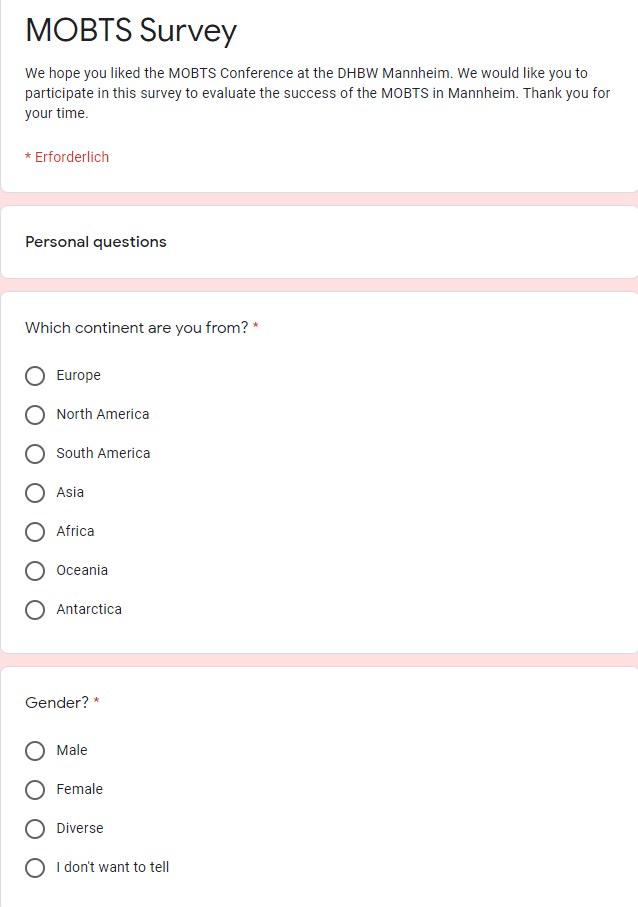
\includegraphics[width=10 cm]{img/survey1.png}
	\caption[MOBTS Umfrage]{MOBTS Umfrage Teil 1}
	\label{fig:survey1}
\end{figure}

\begin{figure}[h]
	\centering
	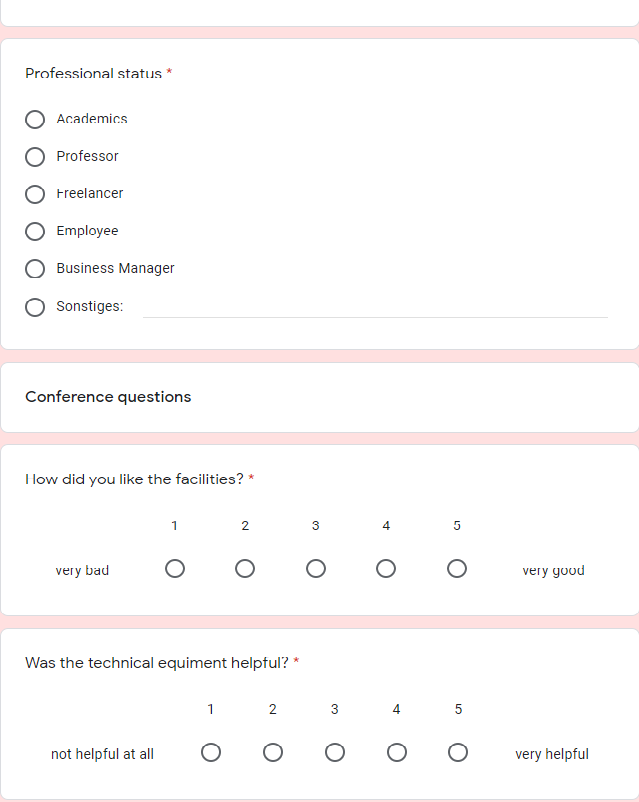
\includegraphics[width=10 cm]{img/survey2.png}
	\caption[MOBTS Umfrage]{MOBTS Umfrage Teil 2}
	\label{fig:survey2}
\end{figure}

\begin{figure}[h]
	\centering
	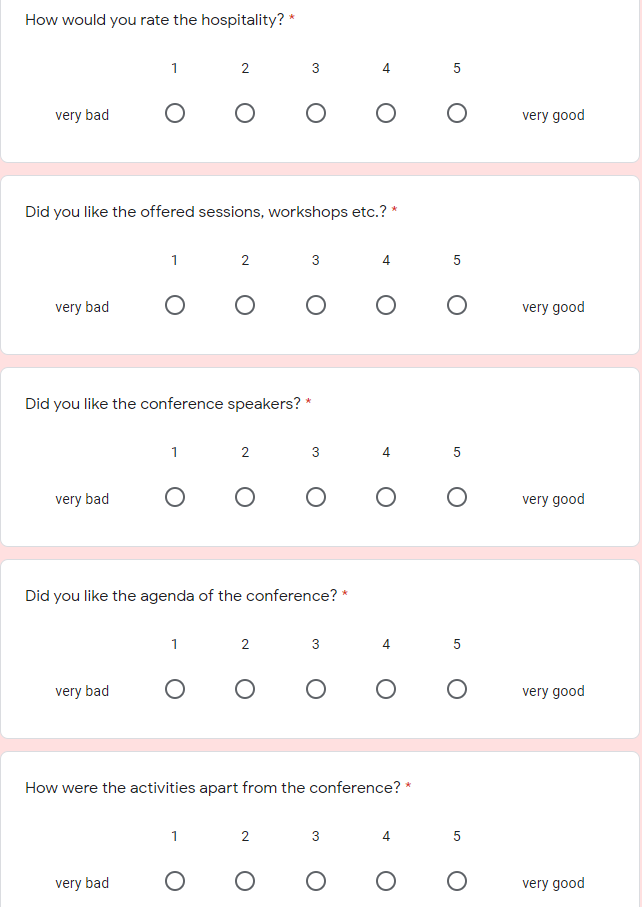
\includegraphics[width=10 cm]{img/survey3.png}
	\caption[MOBTS Umfrage]{MOBTS Umfrage Teil 3}
	\label{fig:survey3}
\end{figure}

\begin{figure}[h]
	\centering
	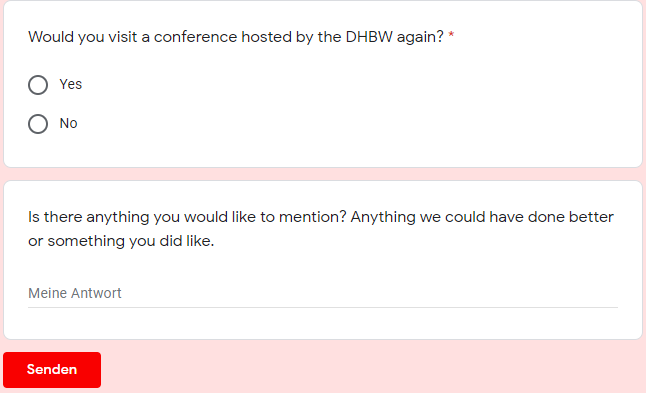
\includegraphics[width=10 cm]{img/survey4.png}
	\caption[MOBTS Umfrage]{MOBTS Umfrage Teil 4}
	\label{fig:survey4}
\end{figure}

\chapter{Catering-Angebot}
\label{app:angebot}

%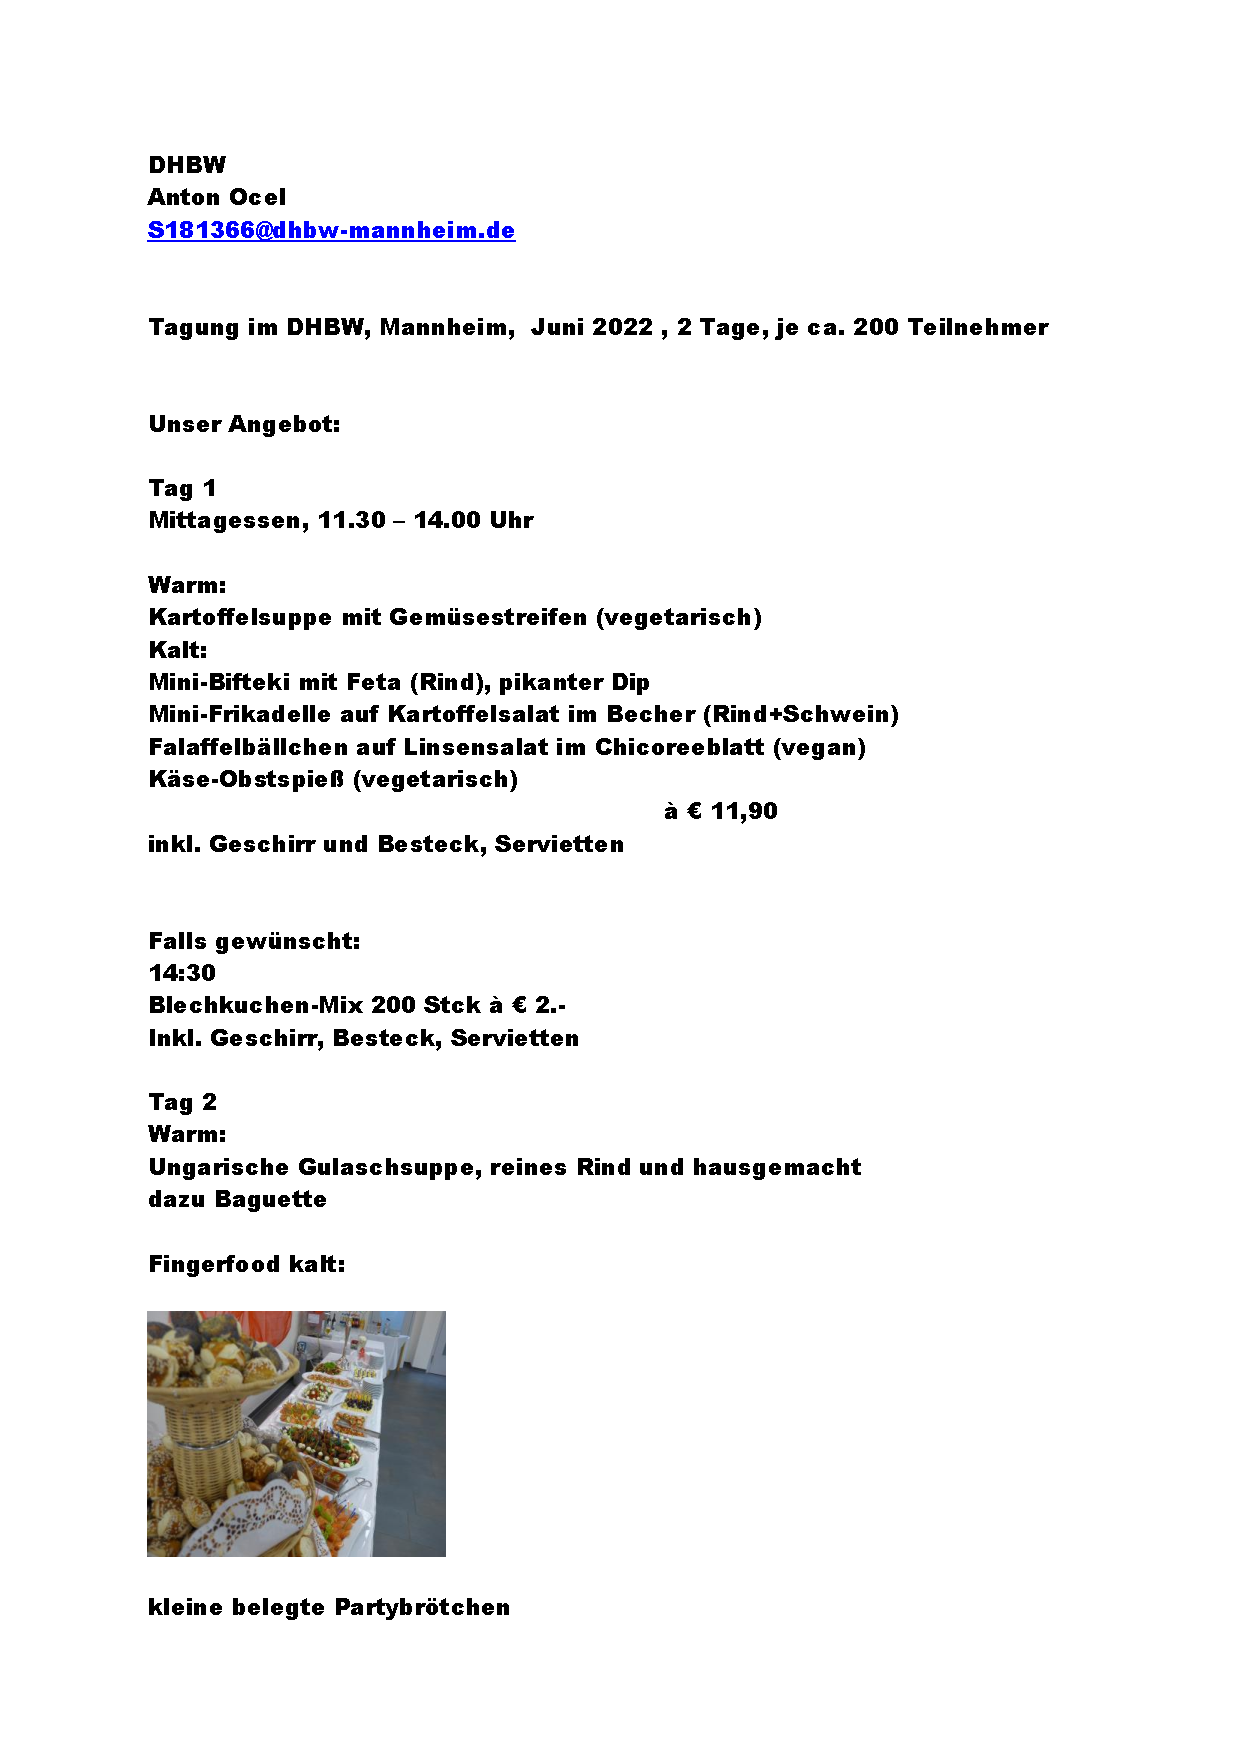
\includepdf[pages=1]{DHBWOcel2x200p22.pdf}



% Ehrenwörtliche Erklärung ewerkl.tex einziehen
% !TEX root =  master.tex

\clearpage
\chapter*{Ehrenwörtliche Erklärung}

% Wird die folgende Zeile auskommentiert, erscheint die ehrenwörtliche
% Erklärung im Inhaltsverzeichnis.

% \addcontentsline{toc}{chapter}{Ehrenwörtliche Erklärung}
Ich versichere hiermit, dass ich die vorliegende Arbeit
 mit dem Thema: \textit{\DerTitelDerArbeit} selbstständig verfasst und keine anderen als die angegebenen Quellen und
Hilfsmittel benutzt habe. Ich versichere zudem,
dass die eingereichte elektronische Fassung mit der gedruckten Fassung übereinstimmt.

\vspace{3cm}
Ort, Datum \hfill \DerAutorDerArbeit



\end{document}